%% LyX 2.3.3 created this file.  For more info, see http://www.lyx.org/.
%% Do not edit unless you really know what you are doing.
\documentclass[oneside,american,english]{amsbook}
\usepackage[LGR,T1]{fontenc}
\usepackage[latin9]{inputenc}
\usepackage{babel}
\usepackage{amstext}
\usepackage{amsthm,amsmath}
\usepackage{amssymb}
\usepackage{cancel}
\usepackage{xcolor}
\usepackage{endnotes,microtype,xspace,graphicx,fancyvrb,multirow}
\PassOptionsToPackage{normalem}{ulem}
\usepackage{ulem}
\usepackage{listings}
\usepackage[tikz]{bclogo}


\usepackage[unicode=true,pdfusetitle,
 bookmarks=true,bookmarksnumbered=false,bookmarksopen=false,
 breaklinks=false,pdfborder={0 0 1},backref=false,colorlinks=false]
 {hyperref}
 
\usepackage{todonotes}
% \usepackage[disable]{todonotes} % to disable all todos
\newcommand{\redtodo}[2][]{\todo[color=red, #1]{#2}}


%  TODOS are here. we ahve /unsure, /change, /info, /improvement. to disable a todo, see how we can add to a todo the option [disable].
\makeatletter

%%%%%%%%%%%%%%%%%%%%%%%%%%%%%% LyX specific LaTeX commands.
\DeclareRobustCommand{\greektext}{%
  \fontencoding{LGR}\selectfont\def\encodingdefault{LGR}}
\DeclareRobustCommand{\textgreek}[1]{\leavevmode{\greektext #1}}
\ProvideTextCommand{\~}{LGR}[1]{\char126#1}


%%%%%%%%%%%%%%%%%%%%%%%%%%%%%% Textclass specific LaTeX commands.
\numberwithin{section}{chapter}
\numberwithin{equation}{section}
\numberwithin{figure}{section}
\theoremstyle{plain}
% \newtheorem{thm}{\protect\theoremname}
% \theoremstyle{definition}
% \newtheorem{xca}[thm]{\protect\exercisename}
% \theoremstyle{definition}
% \newtheorem{sol}[thm]{\protect\solutionname}
% \theoremstyle{remark}
% \newtheorem{rem}[thm]{\protect\remarkname}
% \theoremstyle{definition}
% \newtheorem{defn}[thm]{\protect\definitionname}
% \theoremstyle{definition}
% \newtheorem{example}[thm]{\protect\examplename}

\newtheorem{theorem}{Theorem}[section]
\newtheorem{thm}{Theorem}[theorem]
\newtheorem{corollary}{Corollary}[theorem]
\newtheorem{lemma}[theorem]{Lemma}
\newtheorem{rem}[theorem]{Remark}
\newtheorem{remark}[theorem]{Remark}
\newtheorem{defn}[theorem]{Definition}
\newtheorem{example}[theorem]{Example}
\newtheorem{xca}{Exercise}[section]
% \newtheorem{sol}[xca]{Exercise}



\newcommand{\red}[1]{\textcolor{red}{#1}}

% New commands:

\makeatother

\addto\captionsamerican{\renewcommand{\definitionname}{Definition}}
\addto\captionsamerican{\renewcommand{\examplename}{Example}}
\addto\captionsamerican{\renewcommand{\exercisename}{Exercise}}
\addto\captionsamerican{\renewcommand{\remarkname}{Remark}}
\addto\captionsamerican{\renewcommand{\solutionname}{Solution}}
\addto\captionsamerican{\renewcommand{\theoremname}{Theorem}}
\addto\captionsenglish{\renewcommand{\definitionname}{Definition}}
\addto\captionsenglish{\renewcommand{\examplename}{Example}}
\addto\captionsenglish{\renewcommand{\exercisename}{Exercise}}
\addto\captionsenglish{\renewcommand{\remarkname}{Remark}}
\addto\captionsenglish{\renewcommand{\solutionname}{Solution}}
\addto\captionsenglish{\renewcommand{\theoremname}{Theorem}}
\providecommand{\definitionname}{Definition}
\providecommand{\examplename}{Example}
\providecommand{\exercisename}{Exercise}
\providecommand{\remarkname}{Remark}
\providecommand{\solutionname}{Solution}
\providecommand{\theoremname}{Theorem}

\usepackage{biblatex}
\addbibresource{bib.bib}
\bibliography{bib}


\global\long\def\ball#1{B_{\left|\left|\cdot\right|\right|_{#1}}}%
\global\long\def\C{\mathbb{C}}%
\global\long\def\Q{\mathbb{Q}}%
\global\long\def\F{\mathbb{F}}%
\global\long\def\G{\mathbb{G}}%
\global\long\def\mx{\mathcal{X}}%
\global\long\def\bin#1#2{\binom{#1}{#2}}%
\global\long\def\p#1{\Pr\left[#1\right]}%
\global\long\def\limn#1{\lim\limits _{n\to\infty}\left(#1\right)}%
\global\long\def\one{\mathbbm{1}}%
\global\long\def\cov#1#2{COV\left[#1,#2\right]}%
\global\long\def\E#1{\mathbb{E}\left[#1\right]}%
\global\long\def\enc#1{Enc\left[#1\right]}%
\global\long\def\V#1{var\left[#1\right]}%
\global\long\def\R{\mathbb{R}}%
\global\long\def\N{\mathbb{N}}%
\global\long\def\then{\Rightarrow}%
\global\long\def\norm#1{\left\Vert #1\right\Vert }%
\global\long\def\Z{\mathbb{Z}}%
\global\long\def\from{\leftarrow}%
\global\long\def\getrandom{\overset{_R}{\from}}%


% color for a listing like python code/ algorithm

\definecolor{codegreen}{rgb}{0,0.6,0}
\definecolor{codegray}{rgb}{0.5,0.5,0.5}
\definecolor{codepurple}{rgb}{0.58,0,0.82}
\definecolor{backcolour}{rgb}{0.95,0.95,0.92}

\lstdefinestyle{mystyle}{
    % backgroundcolor=\color{backcolour},   
    commentstyle=\color{codegreen},
    keywordstyle=\color{magenta},
    numberstyle=\tiny\color{codegray},
    stringstyle=\color{codepurple},
    basicstyle=\ttfamily\footnotesize,
    breakatwhitespace=false,         
    breaklines=true,                 
    captionpos=b,                    
    keepspaces=true,                 
    numbers=left,                    
    numbersep=5pt,                  
    showspaces=false,                
    showstringspaces=false,
    showtabs=false,                  
    tabsize=2
}

\lstset{style=mystyle}
\begin{document}

\title{Notes From Students}
\author{Jonathan Weiss}

% \maketitle
\selectlanguage{english}%


\begingroup
\let\newpage\relax
\maketitle
\begin{itemize}
  \item \red{\bf CAUTION! This document was not peer-reviewed and might contain many faults, inaccuracies, grammar issues and typos.}
  \item These notes are a collection of information I've gathered regarding distributed systems,
  cryptography, and math. Mainly intended to
 be a source of knowledge to look back at and get quickly into the
 notions. Some of the items will have sources, and some will simply be proved here.
\end{itemize}
\endgroup



\pagebreak\tableofcontents



\part{Algebraic structures}
This section was motivated by a theorem for polynomial identity, which is used in many cryptography applications:
\begin{lemma}[DeMillo-Lipton-Schwartz-Zippel lemma] 
\label{schawtz-zippel}
Let $p\in \F[x_1,x_2,x_3,\dots, x_n]$ be a non-zero polynomial of a total 
degree $d\ge0$ over a field $\F$. Let $S$ be a finite set of $\F$ and let 
$(r_1,r_2,\dots,r_n)$ be selected at random, \emph{independently and uniformly} from $S$.
Then 
$$ \Pr{[p(r_1,r_2,\dots,r_n)=0]}\le \frac{d}{|S|}$$
\end{lemma}

Unfortunately, this doesn't work over quotient polynomial rings (e.g., instead of
 $\F[x]$, we have $\F[x]/(x^n+1)$).

We'll start learning Algebraic structures in hopes we gain enough insight regarding \ref{schawtz-zippel}.
\chapter{Group theory}

\section{Group}
\begin{defn}
    A \emph{group} is a set $G$ with a binary operation $\cdot :G\times G\to G$ that satisfies the following constraints:
    \begin{itemize}
        \item the operation holds closure: if $x,y\in G$ so is $x\cdot y\in G$.
        \item the operation is associative: $\forall x,y,z\in G$ it holds that $(x\cdot y)\cdot z = x\cdot (y\cdot z)$.
        \item has an identity element: there exists $e\in G$ such that $\forall x\in G x\cdot e = x = e\cdot x$
        \item Every element $x\in G$ has an inverse $x^{-1}\in G$ such that $x\cdot x^{-1} = e = x^{-1} \cdot x$.
    \end{itemize}
\end{defn}

\begin{remark}
    Note that a group can be an additive group or a multiplicative group.
\end{remark}
\begin{example}
    Assume $\F*=F\\{0}$, $(\F*, \cdot, 1)$ is a valid multiplicative group but,
    $(\F, \cdot, 1)$ is not because there is no inverse to $0$ in $\F$.
\end{example}

\begin{defn}
    group $G$ is called \emph{commutative}, or \emph{abelian} if for every $x,y\in G$ $x\cdot y=y\cdot x$ holds.
\end{defn}

\subsection{traits of groups}
let $(G,\cdot,e)$ be a group, thus
\begin{itemize}
    \item $e$ is unique (like in fields).
    \item the inverse of an element is unique.
    \item $\forall x\in G (x^{-1})^{-1}=x$.
    \item $\forall x,y\in G (x\cdot y)^{-1}=y^{-1}\cdot x^{-1}$
\end{itemize}


\begin{defn}
    denote $|G|$ as the \emph{order} of a group - its size.
\end{defn}

\begin{defn}
    denote the order of $x\in G$ to be the minimal $m!=0\in\N$ such that  $x^m=e$. if there is no such $m$, then
    the order of $x$ is infinite.
\end{defn}

\begin{thm}
    Let there a finite group $G$, thus $\forall x\in G$ has a finite order.
\end{thm}

\begin{thm}
    Let $G$ be a group, and let $x\in G$ such that $order(x)=n$, thus $x^m=e$ iff $n|m$.
\end{thm}

\begin{thm}[Fermat's little theorem]
    let there be $x$ and $p$ prime, thus $x^p \equiv x \mod p$
    (and as a result $x^{p-1}\equiv e mod p$).
\end{thm}

\subsection{Subgroups}

\begin{defn}
    Let there be a group $G$, $\emptyset \neq H\subseteq G$  is a \emph{subgroup} if it is a group
     with respect to the same operation of $G$.
\end{defn}
usually, we denote a subgroup with $H\le G$.

\subsection{cosets}



% \section{Motivation}
% \section{Ring theory intro}
% In this chapter, we'll discuss definitions, and theorems (many without proofs) extracted and summed by me from~\cite{galois-book-edinburgh} And HUJI's Algebraic structures 1.


% Historically, the subject of Galois theory was motivated by the desire to solve polynomial equations $p(x)=0$
% where $p(x)=\sum_{i=0}^{n}{a_i\cdot x^{i}}$.
% How do we solve for $x$ with some given degree $d$? we know how to do it for $d\in \{0,1,2,3,4\}$. 
% There was no formal way to solve for $x$ when $d\ge 0$. and it remained an open question for hundred of years.
% Unfortunatly,Raffini and Abel(1823) proved that there is no formula for roots of a quintic using only. $+, -, \times , \div, \sqrt[n]{}$.


% Evariste Galois gave a far more conceptual proof, inventing group theory on the way. 
% He died at 20 in a duel (1831). The paper was only published in 1846.

% \section{Rings and fields}

% \begin{defn}
%     We call a group $R$ a \emph{ring} if it is an abelian group (commutative) whose operation $+$,
%     is called addition, with a second operation $\cdot$ callend multiplication that is 
%     associative, distributive and has a multiplicative identity element.
% \end{defn}

% although it isn't always the case, we will assume all our rings are 
% commutative with a multiplicative identity.

% In terms of fields, a field is always a ring, 
% it assumes more properties on the ggiven group.
% a ring can have subsets which are fields.


% \begin{example}
%     There are many ways of building new rings from old. One of the most fundamental
%      is that from any ring $R$, we can build the ring $R[t]$ of polynomials over
%      $R$ (i'll define it formally later).
% \end{example}

% \begin{defn}
%     Given two rings, $R$ and $S$, a \emph{homomorphism} from $R$ to $S$ is 
%     a function $\phi : R\to S$ satisfying the following equations
    
%     \begin{align*}
%         \phi(x+y) = \phi(x) + \phi(y), && \phi(0)=0  \\
%         \phi(x\cdot y) = \phi(x)\cdot \phi(y), && \phi(1)=1 \textbf{\red{important!}}
%     \end{align*}
% \end{defn}
% Note that we gain $\phi(-x) = -\phi(x)$ too. furthermore, that we switch the multiplicity
% and addition operation to be the one that used in $S$
% that is $\phi(x) \cdot \phi(y)$ elements of $S$, and $x\cdot y$ are elements of $R$.

% lalalala
% \begin{lemma}
%      If for some function $\phi:R\to S$ it holds that: 
%     $\phi(x+y) = \phi(x) + \phi(y)$  and $\phi(x\cdot y) = \phi(x)\cdot \phi(y)$,
%     for all $x,y\in R$ than, $\phi$ is a homomorphism.
% \end{lemma}

% \begin{defn}
%     A sub ring of a ring $R$ is a subset $S \subseteq R$ that contains 0 and \red{1} 
%     and is closed under addition, multiplication and negatives.    
% \end{defn}

% \begin{defn}
%     If $R$ is a ring, we'll denote $R[X]$ the ring of polynomials
%     in $x$ with coefficients in $R$. Formally, an element of $R[X]$ is a finite
%     sum: $$ r_0 + r_1x +r_2x^2 +\dots +r_dx^d$$
%     With $d\in\Z\ge0$.
%     We treat $x$s as symbols, rather than actual values or variables.
%     \red{todo: define poly addition and multiplication}
% \end{defn}

% \begin{remark}[technical but important]
%     a polynomial $f(x)\in R[X]$ defined as $f(x)=\sum_{i=0}^{d}{a_i\cdot x^{i}}$. 
%     can be evaluated as a function over $R$, defining $f:R\to R$ by $f(r)=\sum_{i=0}^{d}{a_i\cdot r^{i}}$
%     However, in this generality, different polynomials can give rise to the same function!
%     \begin{example}
%         $R=\Z \\ 2\Z = {0,1}$ the two different polynomials
%         $f(x)=x, g(x)=x^2$ give rise to the same function $R\to R$.
%     \end{example}
% \end{remark}

% \section{Commutative Algebra}
% In this section we gradually define preliminaries for the schwarts-zippel lemma, 
% and polynomial homomorphism.

% \begin{defn}
%     Let $R$ be a ring. An element $a\in R$ is a \emph{unit} if there exists
%      $b\in R$ such that $a\cdot b = b\cdot a = 1$. The set of all units is denoted by $R^*$.
% \end{defn}

% \red{define zero divisors as well when you have the time}.

% \begin{defn}
%     Let $\alpha_0,\alpha_1,\dots \alpha_m-1\in R$. We call $A=\{\alpha_0,\alpha_1,\dots \alpha_m-1\}$ an exceptional set
%     if and only if $\alpha_i- \alpha_j\in R^*$ for all $i,j\in[m]$ with $i\neq j$. 
%     We define Lenstra constant of $R$ to be the size of the biggest exceptional subset of $R$.
% \end{defn}

% \begin{remark}
%     an exceptional set is a private case of a regular difference set,
%     I will not discuss this here.
% \end{remark}

% Now That we've defined exceptional sets, we can talk about the polynomial evaluation homomorphism:

% \begin{defn}[polynomial evaluation homomorphism]
%     \red{TODO}
% \end{defn}

% Given an exceptional set, one can prove  the following:
% \begin{lemma}[schwarts-zippel over rings~\cite{schwarts-zippel-over-rings}]
%     Let $R$ be a commutative ring and $f: R^n \to R$ be an $n$-variate non-zero 
%     polynomial. Let $A \subseteq R$ be an exceptional set. Then
%     $$ \Pr_{x\leftarrow A^n}{[f(x)=0]} \leq \frac{\text{deg} f}{|A|}$$
% \end{lemma}


\part{Algorithms}
\part{Algorithms}

\chapter{Polynomial Algorithms}\label{polynomials}


\section{Coefficient Representation}\label{polynomials:coeffcient-pres}
A coefficient representation of a polynomial $P(x)$ is a vector of coefficients 
$a=(a_0,a_1,\dots, a_{n-1})$.
In coefficient representation, we can evaluate or add a polynomial in $O(n)$ time. 
unfortunately multiplying two polynomials takes $O(n^2)$.
The operation of multiplying two polynomials $a,b$ is called convolution $c=a\otimes b$.
\todo{Define coefficient representation mroe formally}

\section{Polynomial evaluation}
Polynomial evaluation is the process of computing the value of a polynomial at a given point.
This is a fundamental operation in many algorithms and applications. 
There are several methods to evaluate polynomials, with varying levels of efficiency.
Before we delve into the methods, we define what is evaluation of a polynomial and a polynomial evaluation map.

\begin{defn} \label{def:poly-eval}
  For any polynomial $P$ in $Z_q[X]$ and any element $a$ in $Z_q$,
  the substitution of $X$ with $a$ in $P$ defines an element of $Z_q$, which is denoted $P(a)$.
  This element is obtained by carrying on in $Z_q$ after the substitution of the operations indicated by 
  the expression of the polynomial.
  We call this action polynomial evaluation of $P$ at $a$.
\end{defn}

Now that we've defined the evaluation of a polynomial, it is important to state that formally, polynomials aren't functions. 
Thus to evaluate a polynomial at a point, we need to define a function that receives a polynomial and a point and returns the evaluation.
\begin{defn}
  A polynomial evaluation map is a function $f_r:Z_q[X]\to Z_q$ such that for every polynomial $P$ and $r\in Z_q$,
  $f_r(P)=P(r)$.
\end{defn}

This notation of polynomial evaluation maps is crucial to reason about polynomials, their evaluation, 
and proving properties. For instance, assume a matrix $M$ and a vector $v$ with polynomials entries in $\Z_q[x]$.
It isn't clear straight away that $f_r(M\cdot v) = f_r(M)\cdot f_r(v)$. In fact, there are algebraic 
structures where this above equation is false. 
Thus, to claim the above statement we need to define ring homomorphisms, and prove that $f_r$ is a ring homomorphism.

\begin{defn}
  A ring homomorphism is a function $f:R\to S$ between two rings $R$ and $S$ such that for every $a,b\in R$:
  \begin{align}
    &f(a+b)=f(a)+f(b)\\
    &f(a\cdot b)=f(a)\cdot f(b) \\
    &f(1_R)=1_S
  \end{align}
   Where $1_R$ and $1_S$ are the multiplicative identities of $R$ and $S$ respectively.
\end{defn}

Fortunately, for every point in $\Z_q[X]$, we can construct a polynomial evaluation map that is 
a ring homomorphism (prove this to ensure you understand the reasoning behind it).
Consequently, we can assert that $f_r(M\cdot v) = f_r(M)\cdot f_r(v)$.

\subsection{Evaluation Algorithms}
Evaluating a polynomial at a point is a straightforward process.
Substituting the point for $X$ in the polynomial gives the result. 
However, Horner's rule offers a more efficient method.

Horner's rule reduces the number of multiplications required to evaluate the polynomial.
It rewrites the polynomial in a nested form, making computation more efficient.

To apply Horner's rule to evaluate a polynomial $P(x) = a_0 + a_1x + a_2x^2 + \dots + a_nx^n$ at a 
point $x = r$, follow these steps:

\begin{lstlisting}[language=Python,
  caption={fft algorithm in python}
]
def horner(p: List[int], r: int) -> int:
    result = p[-1]
    for i in range(len(p) - 2, -1, -1): # iterate from n-1 to 0
        result = result * r + p[i] # result = ((((....)x+a_3)x+a_2)x+a_1)x +a_0 = p(r)
    return result
\end{lstlisting}\label{algorithm:polynomial:evaluation}


\section{Coefficient vs Point-Value representation}\label{polynomials:point-val-representation}
We've defined one representation for polynomials, the coefficient representation~\ref{polynomials:coeffcient-pres},
But there is another representation, which is used in numerous algorithms (e.g.,~\ref{schawtz-zippel},\ref{polynomial:multiplication}):


A point-value representation of a polynomial $P(x)$ of degree-bound $n$ is a set of $n+1$ point-value pairs.
$ \{ (x_0,P(x_0)),\dots , (x_{n}, P(x_{n})) \}$, which uniquely defines it.

\begin{theorem}[Uniqueness of an interpolating polynomial]
  For any set $ \{ (x_0,P(x_0)),\dots , (x_{n}, P(x_{n})) \}$ of $n+1$
  point-value pairs such that all the $x_k$ values are distinct,
  there is a unique polynomial $P(x)$ of degree-bound $n$ such that
  $y_k = P(x_k)$. for $k\in[n]$ 
\end{theorem}

\begin{proof}
  \sloppy{
  So let there be a polynomial $p(x) \neq 0$ of degree 
  $n$ and a set $ \{ (x_0,P(x_0)),\dots , (x_{n}, P(x_{n})) \}$
  of points representing it. Let us assume in contradication that there exists $q(x)\neq p(x)$ and it also happens
  that $p(x_0)=q(x_0), \dots, p(x_n)=q(x_n)$. That is, there is another polynomial that is evaluated to the same points,
  making the representation non-unique.

  So if such $q(x)$ exists, we can create a new polynomial $(p-q)(x)$, notice that $(p-q)$ is also of degree $n$.
  $x_i$ is a root $0\le i\le n$ of $(p-q)(x)$, since $(p-q)(x_i)=p(x_i)-q(x_i)$, thus it has $n+1$ roots.
  This is a contradication to the fundamental theorem of algebra \todo{cite}, that is, a polynomial $p(x)\neq 0$ 
  of degree $n$ has at most $n$ roots. }
\end{proof}

Now that we know that this representation is unique, I'll claim without proof that
there is a mapping that is both injective and surjective (bijective) from both representations.
Thus these both know representations are isomorphic.

\section{Polynomial Modulo}
\red{TODO}
\section{Polynomial Identity Testing (SZ)}\label{schawtz-zippel}
In this section, we talk about identity testing, 
and some issues involving this subject.

Given two polynomials $P(x)$ and $Q(x)$ of the same degree $d$, 
how do we prove these are the same polynomials?
We can calculate it and check $d$ points on each polynomial 
since each polynomial can be solely defined by its point-value representation\ref{polynomials:point-val-representation}.


Schwartz-Zippel \cite{SZ} made this notion much more efficient 
(and complete since they discuss multivariate polynomials).
By choosing a random point for evaluating each polynomial, we can 
be almost entirely certain 
whether the polynomials are equal or not.

\begin{theorem}
 Let $P(x)$ be a non-zero polynomial of total degree $d$ over 
 an integral domain $R$. Let $S$ be a finite subset of $R$, and let $r$
 be a selected random number from $S$. Then
  $\Pr [P(x)=0]\le \frac{deg(p(x))}{|S|}$.
\end{theorem}
\begin{proof}
  $P(x)$ is a polynomial, from the fundamental theorem of algebra\cite{Aigner2010} it has 
 at most $d$ roots. Thus, choosing some random point $r$,
  $\Pr [P(r)=0]\le \frac{d}{|S|}$. 
\end{proof}


Given this notion, one can easily extrapolate this idea and create a method 
to check whether $P(x)\cdot Q(x)$ is equal to some given $Z(x)$: 
choose a random number $r$, and evaluate $P(r)\cdot Q(r) - Z(r)$.
if this expression equates to $0$, then $P(x)\cdot Q(x)=Z(x)$ with overwhelming 
probability (depending on the size of $Z_q$).

\subsection{Troubled waters in $Z_q[X]/F(X)$}
Given the above method, we can investigate new and upcoming ideas on numerous
problems (see  \cite{sz-usage2} and \red{fpir- to be published}).
The unlucky ones might encounter a troubling problem.
While SZ works quite well over fields and rings,
One would quickly find out that more complex algebraic structures do not 
bend so easily to this powerful technique.

For instance, consider the following quotient polynomial rings $R_q=Z_q[X]/(X^n+1)$,
choose two random polynomials from $R_q$, and try the method of testing above.
It is highly likely that for some random $r$, $P(r)\cdot Q(r) \ne (PQ \mod (X^n+1))(r)$.

This issue arises because not every point $r\in Z_q$ can be used to construct a
polynomial evaluation map $f_r$ (refer to \autoref{def:poly-eval}) 
over $R_q$ such that $f_r$ is a ring homomorphism. 
Consequently, certain values of $r$ will not be compatible with the Schwartz-Zippel method.
In other words, $f_r(P\cdot Q) \neq f_r(P)\cdot f_r(Q)$.


\paragraph{Finding valuable points}

Fortunately, there are some points $r\in \Z_q$ which can be used to create polynomial evaluation maps that 
are ring homomorphisms.
\begin{thm}
  Let $R_q=Z_q[X]/F(X)$ and let $r\in Z_q$. If $F(r)=0$ then $f_r$ is a ring homomorphism.
\end{thm}
\begin{proof}
  $f_r$ preserve the multiplicativeidentity: $f_r(1_{R_q}) = 1(r)=1$.
  Every $f_r$ preserver addition.
  preserving multiplication:
  Let there be $P(X), Q(X) \in R_q$. 
  By definition $P(X)\cdot Q(X) \mod F(X) = P(X)\cdot Q(X) \lfloor \frac{P(X)\cdot Q(X)}{F(X)} \rfloor \cdot F(X)$,
  so $f_r(P(X)\cdot Q(X))= f_r(P(X))cdot f_r(Q(X)) - f_r(\lfloor  \frac{P(X)\cdot Q(X)}{F(X)} \rfloor)\cdot f_r(F(X))$.
  Because $f_r$ is an evaluation map, $f_r(\lfloor  \frac{P(X)\cdot Q(X)}{F(X)} \rfloor)=z$ where is some unknown integral from $Z_q$.
  then $f_r(P(X)\cdot Q(X)) =P(r)\cdot Q(r) - z \cdot 0= P(r)\cdot Q(r)$, as wanted.
\end{proof}

So, by finding the roots of $F(X)$, we can identify potential values where 
the SZ algorithm continues to function effectively. 
However, this set is quite limited (consider the maximum number of roots of the polynomial $F(X)$).

\section{Polynomial addition}\label{polynomials:addition}
\section{Fast Polynomial Multiplications}\label{polynomial:multiplication}\label{section:fft}

We know how to add two polynomials as efficient as possible~\ref{polynomials:addition},
but the simple definition of polynomial multiplication isn't as efficient, and demand $O(n^2)$.
Many complex algorithms make use of polynomial multiplication, and as a result, the algortihm 
we are going to describe was announced as one of the top 10 Algorithms of 20th
Century by the IEEE magazine Computing in Science and Engineering.\cite{814652}


We begin by remembering the point-value representation~\ref{polynomials:point-val-representation}.
In this representation, once can perform both addition and multiplication between two polynomials 
by performing point to point operations (similar to addition in coefficient representation)\todo{provide proof?}.
As a result multiplication and addition in this representation cost $O(n)$.


The naive algorithm of moving from coefficient representation to point-value representation
requires evaluating the polynomials $n+1$ times, and as a result runs in $O(n^2)$.
Thus, to perform polynomial multiplication we'll begin with finding a clever and fast way to move between representations.
\subsection{FFT}
Luckily there is a way to move to and from both representations quickly using the \emph{roots of unity}.

\begin{defn}
An $n$th root of unity is a complex number $\omega$ such that
$\omega^n =1$.
\end{defn}

There are exactly $n$ roots of unity $e^{2\pi i k/n}$ for $k\in[n-1]$ 
($e^{iu}= \cos{u}+i \sin{u}$).

The value $\omega_n=e^{2\pi i/n}$ is the \emph{principal nth root of unity}.
all other roots of unity are powers of $\omega_n$:
 $\omega_n^0, \omega_n^1, \omega_n^2,\dots, \omega_n^{n-1}$.

FFT takes special advantage that these values have special properties.
\begin{lemma}[roots of unity]\label{roots-of-unity-property}
If $z$ is an nth root of unity, then $ a \equiv b \mod n \Rightarrow z^a = z^b$.
\end{lemma}
meaning that $\omega_n^a = \omega_n^b$. one can label specific points on the unit circle over $\C$.

\paragraph{Why is that important?}

In the simplest of cases, we are going to evaluate the polynomial over the following
points $ \{\omega_n^0, \omega_n^1, \omega_n^2,\dots, \omega_n^{n-1}\}$.
Let us view the polynomial evaluation over $n$ such points as a matrix, this presentation
might help the reader see some similarities:


$$
\begin{pmatrix}
  y_0\\
  y_1\\
  \vdots \\
  y_{n-1}\\
\end{pmatrix}
=
\begin{pmatrix}
  1 & x_0 & x_0^2 ,\dots\\
  1 & x_1 & x_1^2, \dots,\\
  \vdots & \vdots & \vdots & \ddots & \\
  1 & x_{n-1} & x_{n-1}^2, \dots,\\
 \end{pmatrix}
 \cdot 
\begin{pmatrix}
  a_0\\
  a_1\\
  \vdots \\
  a_{n-1}\\
\end{pmatrix}
 $$

 Now, let us assign the values:

 \label{dft-matrix}
 $$
\begin{pmatrix}
  p(\omega_n^0)\\
  p(\omega_n^1)\\
  \vdots \\
  \omega_n^2\\
\end{pmatrix}
=
\begin{pmatrix}
  1 & (\omega_n^0)^1 & (\omega_n^0)^2 ,\dots ,(\omega_n^0)^{n-1}\\
  1 & (\omega_n^1)^1 & (\omega_n^1)^2, \dots, (\omega_n^1)^{n-1}\\
  \vdots & \vdots & \vdots & \ddots & \\
  1 & (\omega_n^{n-1}) & (\omega_n^{n-1})^2, \dots,(\omega_n^{n-1})^{n-1}\\
 \end{pmatrix}
 \cdot 
\begin{pmatrix}
  a_0\\
  a_1\\
  \vdots \\
  a_{n-1}\\
\end{pmatrix}
 $$

 The keen looker can see that we can reuse values in this matrix.
 for example, let us look at $(\omega_n^{n-1})^{n-1}$ using \ref{roots-of-unity-property}
 $(\omega_n^{n-1})^{n-1} = (\omega_n)^{n*n-2n+1}=(\omega_n)^{0+0+1}$.  

 Thus we gain a matrix with heavy symmetry, which the FFT can use.

\paragraph{fft main idea}
The FFT method employs a divide-and-conquer strategy, 
using the even-indexed and odd-indexed coefficients of $A(x)$
separately to define the two new polynomials $A^{[0]}(x)$ and $A^{[1]}(x)$ of degree-bound $n/2$.

\begin{align}
  &A^{[0]}(x) =  a_0 +a_2x + a_4x^2 + \dots + a_{n-2}x^{n/2-1}\\
  &A^{[1]}(x) =  a_1 +a_3x + a_5x^2 + \dots + a_{n-1}x^{n/2-1}.
\end{align}


It follows that $A(x)=A^{[0]}(x^2) + x\cdot A^{[1]}(x^2)$.

Thus, the problem of evaluating $A(x)$ at 
$\omega_n^0, \omega_n^1, \omega_n^2,\dots, \omega_n^{n-1}$ 
reduces to evaluating the degree-bound $n/2$ polynomials  $A^{[0]}(x)$ and $A^{[1]}(x)$ at the points
$$(\omega_n^0)^2, (\omega_n^1)^2,\dots, (\omega_n^{n-1})^2$$
and then combining the results according to $A(x)=A^{[0]}(x^2) + x\cdot A^{[1]}(x^2)$.


Using the properties of the root of unity, 
the above values consist not of $n$ distinct values but only of the $n/2$
 complex ($n/2$)th roots of unity, with each root occurring exactly twice!
These subproblems have the same form as the original problem but are half the size.
We can continue in this manner until we evaluate the full polynomial on $n$ distinct values.


\subsection{putting it all together}
\red{there might be some miscalculations here, but the idea is solid.}
As we've seen we can create a matrix with heavy symmetry, called the DFT matrix. 
now, we'd want to capitalize on that and create a recursive algorithm.
To do so, instead of the regular polynomial assignment we've seen above using a matrix,  
we'll shuffle things a bit according to the divide-and-conquer approach from above
$$
F_n \cdot p(x) = 
\begin{pmatrix}
  I_{ \frac{n}{2}} & D_{\frac{n}{2}} \\
  I_{ \frac{n}{2}} & -D_{\frac{n}{2}}
 \end{pmatrix}
 \cdot 
 \begin{pmatrix}
  F_{ \frac{n}{2}} & 0 \\
  0 & F_{ \frac{n}{2}} 
\end{pmatrix}
\cdot 
\begin{pmatrix}
  p_{\text{even coefficient}} \\
  p_{\text{odd coefficient}}
\end{pmatrix}
 $$

 where $F_n$ is the matrix of assignment we've seen in ~\ref{dft-matrix}, and 
 $D_n$ is the following diagonal matrix $$
 \begin{pmatrix}
  1 & 0 &0  & \dots& 0 \\
  0 & \omega_n^1 &0  & \dots& 0 \\
  1 & 0  &\omega_n^2  & \dots& 0 \\
  \vdots & \vdots & \vdots & \vdots &  \\
  0 & 0  &0  & \dots& \omega_n^n-1 \\
 \end{pmatrix} $$


 We can continue this process recursively, to get what we want.
 In each recursive level, the algorithm does at most $O(n)$ work (i.e., multiplying by sparse matrices),
  and due to the logarithmic depth of the recursion, we get $O(n\log{n})$.
x
\label{algorithm:fft}
  \begin{lstlisting}[language=Python,
    caption={fft algorithm in python}
  ]
import numpy as np

def fft(p: np.ndarray) -> np.ndarray:
    n = len(p)
    if n == 1:
        return p
    omega = np.exp(2 * np.pi * 1j / n)

    p_even, p_odd = p[::2], p[1::2] 
    ye, yo = fft(p_even), fft(p_odd)

    # mult the structured left matrix with the recursive result.
    # O(n) work comes from here.
    y = np.zeros(n, dtype=np.complex128)
    for k in range(n // 2):
        y[k] = ye[k] + omega ** k * yo[k]
        y[k + n // 2] = ye[k] - omega ** k * yo[k]
    return y
    \end{lstlisting}
    
    \begin{remark}[Summary]
      Notice that to achieve this result, we needed to reduce the polynomial into
      even and odd parts, and then adjust the assignment matrix using
      the properties of roots of unity. Each part is important in its own way.
    \end{remark}
\subsection{Inverse FFT}\label{ifft}

The DFT matrix is invertible.
Thus one can solve for the vector of coefficients,
by simply inverting the matrix in~\ref{dft-matrix}.

Fortunately, with little tricks we can adjust the inverse of the DFT matrix such that
we can use the same algorithm as above, but instead of
$\omega^k$ we'll use $\omega^{-k}$, and after we are done with the FFT
algorithm, we'll need to normalize it by dividing every coefficient element
by $N$ the size of the polynomial.

 \begin{corollary}
  For FFT, DFT, and NTT we must use specific values to gain speedy interpolation and
  evaluation of the polynomial. 
 \end{corollary}{Conclusin:}
 
\subsection{Number Theoretic Transform (NTT)}\label{ntt}

NTT is a specialized version of the discrete Fourier transform,
in which the coefficients of the polynomial are members of a finite field (or ring)
 containing the right roots of unity.
It can be viewed as an exact version of the complex DFT, avoiding 
round-off errors for exact convolutions of integer sequences.
While Gauss used similar techniques already in~\cite{gaussfft}, laying the groundwork 
for modern FFT algorithms to compute the DFT, and therefore the NTT, 
is usually attributed to Cooley and Tukey's seminal paper \cite{fft}.

NTT can use the same FFT algorithms but requires a 
different DFT matrix~\ref{dft-matrix}.

This fact lies in the foundational theorem of NTT:
\begin{thm}[\cite{ntt}]
  A length $N$ transform having the DFT structure will
  implement cyclic convolution if and only if there exists an 
  inverse of N and an element $\alpha$,
  a root of unity of order $N$ , i.e., $N$ is the least 
  positive integer such that $\alpha^N =1$.
\end{thm}
This is a very general result applying to both \emph{rings and fields} that are
finite or infinite.

It is important to note that $N$ also applies to the length of our polynomial.

\subsubsection{Preliminaries}
I will describe everything in terms of fields, but essentially all of this can be easily generalised to rings 
using the Chinese Remainder Theorem (CRT), as shown below.
\paragraph{\bf Finding Roots of Unity (In Field)}
As described above, an $n$-th root of unity, is an element $\alpha\in Z_q$ 
such that $\alpha^n =1  \mod q $, and for every $0<k<n$ $\alpha^k \neq 1 \mod q$.

\paragraph{Finding roots of unity in a field}

\begin{thm}
  Let $g\in GF(q)$ be a generator, thus
  $\omega_0=g^{(q-1)/n}$ is an $n$-th root of unity.
\end{thm}
\begin{proof}
  \sloppy{
  relying on \autoref{fermats-little-theorem}, we know that $g^{q-1}=1 \mod q$.
  So $\omega_0^n=(g^{(q-1)/n})^n=1$, now we just need to explain away why $\omega_0^k \ne 1$ for 
  every $0<k<n$.
  Let us assume in contradiction that there exists some $k<n$ such that $\omega_0^k=1$, then 
  $\omega_0^k=g^{(q-1/n)\cdot k}=1$, more specifically, $g^c=1$ for $c<q-1$. thus, we have a 
  cycle $(1,g,g^1,...g^{c-1})$, which is less than $q-1$ elements, meaning that $g$ is not 
  a generator, in contradiction.
  }
\end{proof}

Now that we found the first root of unity,
we can find the rest by computing the powers of $\omega_0$ up to $n$.


But how do we find the generator to begin with? 
There is a randomised algorithm to find a generator in an expected 
$\approx O(\sqrt{q-1})+O(\log^2{q}\cdot \log (\log(q-1)))$ time for small primes.
For larger primes it'll longer, but it is still feasible ($O(e^{\log q-1})$).

The algorithm itself is based on factorising $q-1$ into prime factors, and then
check that a random number $g$ is a generator by ensuring $g^{(p-1)/p_i} \not\equiv 1$
for each $p_i$ prime factor of $q-1$ (where $q$ is the field's prime order).


\paragraph{Neat Trick}
\todo{This section would have saved me days of work, had I known it before.}
One can make use of these roots of unity to find the roots of $X^n+1$ and $X^n-1$.
Finding the roots of $X^n-1$ is from the definition! 
Every n-th root of unity is a root of $X^n-1$: $(\omega^k)^n=(\omega^n)^k=1^k=1$.
Substitute $X$ with any n-th root of unity, and you'll get $1-1=0$.

Finding the roots of $X^n+1$ is a bit more tricky,
but it can be done by finding the roots of $X^{2n}-1$ (which should be easy
as we've shown above):
First let's recall that $X^{2n}-1=(X^n+1)(X^n-1)$, then we notice that
we have $n$ roots of $X^n-1$,
and $n$ roots of $X^n+1$. So every one of the roots of $X^{2n}-1$ that is
not a root of $X^n-1$ is a root of $X^n+1$.
How do we find the roots of $X^{2n}-1$? Those are the $2n$-th roots of unity, 
which are easy to find!

\paragraph{\bf Finding Inverse}
\todo{explain Bezout's algorithm, majorly known as the extended Euclidean algorithm.}


\paragraph{\bf Chinese Remainder Theorem (CRT) For Dummies}
CRT is a way of representing elements $x\in Z_q$ (
  where $q=p_1,p_2,\dots,p_k$ and $p_i\in\text{Primes}$)
such that the $x_{CRT}$ is a single and unique representation of $x$ using the 
remainders of each of the prime factors constructing $q$:

$$ x_{CRT} = (x\mod p_1, x\mod p_2 ,\dots x\mod p_k ) $$



Because it is a unique representation, given $x_{CRT}$ and the list of
 primes $(p_1,p_2,\dots,p_k)$ there is an algorithm to solve for $x \in Z_q$
 (i.e., find $x \mod q$).


Another important thing to notice is that if  $x=1 \mod q$
 then $x_{CRT}= (1,1,1,\dots,1)$.


There is more to it honestly, but for our cause, it's enough.

\subsubsection{Putting it all together}

\paragraph[NTT Over Finite Fields]{\bf NTT Over Finite Fields} \label{ntt-field}
When working over a field $GF(p)$ such that $p$ is prime,
the maximal $N$, the array of coefficients representing a
polynomial, is $N_{max}=p-1$, and $N$ is a valid size for NTT
 in this field iff $N|p-1$ (\cite[III. number theoretic transforms]{ntt}). 


To compute the NTT over $GF(p)$, find the $n$th root of unity in $GF(p)$,
 then run any FFT algorithm mod $p$ using the roots
of unity for each level of the recursion.

That is, find $\omega_n=\alpha$ such that $\alpha^N=1 \mod p$, 
then run the (almost) same algorithm in \nameref{algorithm:fft}, 
but change line 7 such that omega is now the $n$-th root of unity in $GF(p)$, and
all operations in the algorithm are now $\mod p$.

\paragraph{\bf iNTT}
Just like in \nameref{ifft}, but to calculate $\omega^-1$, we'll
use Bezout's algorithm to find the inverse of every element ($x^-1$).



\paragraph[short]{\bf NTT over Rings}
Let $Z_M$ represent a ring of integers ${0,1,2,\dots , M-1}$,
with arithmetics mod $M$.
Where $M$ is constructed the following unique prime factorization
$M=p_{1}^{r_1}\cdot  p_{2}^{r_2} \cdots p_{\ell}^{r_\ell}$
and $p_i$'s are distinct primes (see \cite[NTT sec. III][]{ntt}
 for further explanations).

For NTT to work, the following must hold $\bf N|L(M)$
where $L(M)$ is the greatest common
divisor (gcd) of the $(p_{i}-1)$. That is, 
$L(M):= gcd\{p_1-1,p_2-1,\dots\}$

essentially it means we want $ N$ to divide $p_i-1$.

\begin{corollary}
  $L(M)=N_{max}$. i.e., it defines the maximal $N$ 
  such that we can apply NTT.  
\end{corollary}

Now, Once $M$ and $N$ are known, to perform NTT we just need to be able to find 
$N$-th root of unity. but it's quite hard to find one in $Z_M$.
Luckily, we know it is feasible to do so in a prime field. 
So, let's find $\alpha_i$, the $N$-th root of unity for every $p_i$.
Once we find all of these roots of unity, we know that $\alpha_i^N=1 \mod p_i$ for every $i$.
In other words, $N$ is the least positive integer such that
\begin{align*}
  &\alpha_{CRT}^N = (\alpha_1^N \mod p_1=1, \alpha_2^N \mod p_2=1,\dots)= (1,1,\dots)
\end{align*}

and according to CRT $\alpha^N=1 \mod M$. Thus, solving for $\alpha$ 
means we'll be able to find the $N$-th root of unity in $Z_M$.

The algorithm remains the same as in \nameref{ntt-field} from here on.

\paragraph{Special Features}
Applying the NTT transform provides a cyclic convolution, computing 
$c = a \cdot b \mod (X^n + 1)$  with two polynomials $a$ and $b$ would require 
applying the NTT of length $2n$ and thus $n$ zeros to be appended to each input;
this effectively doubles the length of the inputs and also requires the computation of 
an explicit reduction modulo $X^n +1$. 
To avoid these issues, one can exploit the \emph{negative wrapped convolution} \cite{negantt}.

This exploitation allows us to perform $NTT$ without expanding to $2n$ parameters!
meaning we can send less bandwidth over the network, and perform fewer computations too. 
This trick can be seen in \cite{SEAL}.

\section{Reed-Solomon}
It is fairly simple, but effective algorithm to encode words and be able to deal with erasurs.
\subsection{Naive solution}
assuming we decide we want our words to be of size $k=4$, and we add additional two redundancies $n=6$. 
Thus to send it we'll do the following: given a word vector, we'll treat it as coefficients values of a 
polynomial of degree $k-1$ (because we have k coefficients its a k-1 degree poly), then to encode it, we'll evaluate it on the following $x$ values: $(-1,0,1,2,\dots n)$.


Now given the 6 values that we received over the network we can decode it as follows: 
We go over every group of 4 points, and try to reconstruct the polynomial. 

the polynomial we've reconstructed the most is the correct one.

\subsection{Systematic Reed-Solomon}
Assuming we want to be able to correct up to $s$ values, we'd need at least $2s$ redundant symbols.
So if $k=4$, and $n=6$, we can only recover a single byte.

It won't work for larger values, like $k=223$, $n=255$ which is a popular value for reed-solomon.
(Meaning we add 32 more symbols to our message, so we can repair 16 symbols in total).

The previous algorithm will work, but we'd need to send different values then 
the original message. It would be best to send $Message||\text{addition code word}$.
that way,we might be able to avoid reconstruction if we can find quickly that there was no error.

this is called a Systematic code. 

\part{Cryptography}
\begin{definition}[$\lambda$-bit strength]
  Defining the strength of security is complex. NIST decided that $\lambda$-bit security 
  means that for any kind of known attack, the attacker would need at least $2^{\lambda}$
  operations to break the scheme.

  Where each operation is defined as a single op over the specified field or ring.
  For instance, over an elliptic curve, either multiplication or additions are assumed to 
  take 1 single CPU cycle.
  
\end{definition}

\chapter{Basics}
\section{Diffie-Helman}
Diffie-Helman relies on the following assumption.

\begin{definition} [Decisional Diffie-Helman (DDH)]\label{DDH}
  Consider a (multiplicative) cyclic group $\G$ of order $q$ and with generator $g$. 
  Given $g^a$ and $g^b$ for $a,b\in_R Z_q$ then $(g^a,g^b,g^{ab})$, $(g^a,g^b,g^{ab})$ are computationally indistinguishable:

  $$ \Pr[A((g^a,g^b,g^{ab}))=1] - \Pr[A(g^a,g^b,g^{c})=1]\le \delta(n)$$
  for $\delta(n)$ a negligable function in $n$.
\end{definition}

Given this assumption, which most of the world takes as FACT (until proven otherwise), then
we can define the key exchange protocol.
\paragraph{DH key exchange}
While not safe against man-in-the-middle attacks, DH is an excellent way to create a shared secret.
The protocol goes as follows.
Assume we have two players, Alice and Bob, both know the other's public key $g^a$ and $g^b$ respectfully,
each takes their secret key $a$ or $b$ and raises the other's public key to the power of $a$ (or $b$).
Both now hold $g^{ab}$, and no one else can compute it since they don't know the secret of either Bob or Alice.

Alice and Bob can use this new number/ or elliptic curve point $g^{ab}$ as a private key for
a symmetric encryption scheme like AES (e.g., $symKey=Hash(g^{ab})$).


\chapter{Elliptic curves}
Taken from \emph{A Graduate Course in Applied Cryptography, Dan Boneh and Victor Shoup}

The best-known discrete log algorithm in an elliptic curve group of size $q$ runs in time $O(\sqrt{q})$. 
This means that to provide security comparable to AES-128, it suffices to use a group of size $q \approx 2^{256}$ 
so that the time to compute discrete log is $\sqrt{q} \approx 2^{128}$.

\section{a bit of history on elliptic curves}
\sloppy{
Elliptic curves come up naturally in several branches of mathematics.
Here we will follow their development as a branch of arithmetic (the study of rational numbers).
Diophantus, a greek mathematician who lived in Alexandria in the third century, was interested 
in the following problem: Given a bivariate polynomial equation, $f(x,y)=0$ find 
rational points satisfying the equation. That is, find $P=(x,y)$ such that $x,y\in\mathbb{Q}$.
Diophantus wrote a series of influential books on this subject, called the \emph{Arithmetica}, of which six survived.
Much of Arithmathica studies integer and rational solutions of quadratic equations.
For example, one of the first problems in the books regarding elliptic curves is to find $(x,y) \in \Q$
 that satisfy the equation $$ y^{2}=x^3 - x + 9$$
The method invented to answer this question secures most Internet traffic worldwide.
One can easily verify that the following points are on the curve $(0, \pm3), (1, \pm3), (-1, \pm 3)$.
Diophantus developed a method similar to \underline{chord method}:
Given two rational points $U$ and $V$ on the curve, where $U\neq -V$, we can pass a line through them,
 and this line must intersect the curve at a third rational point $W$. 
The chord method was rediscovered several times over the centuries, but it finally stuck with the work of Poincare.

Poincare defines the sum of $U, V$, denoted $U \boxplus V$ as $U \boxplus V := -W$
Diophantus' method, the \emph{tangent method} is another way to build a new rational point from a given rational point. 
We should later see that the method corresponds to adding the point $P$ to itself: $P\boxplus P$.}

\section{elliptic curves over finite fields}
We are primarily interested in elliptic curves over finite fields for cryptographic applications.
\begin{definition}
  Let $p >3 $ be a prime. An \textbf{elliptic curve} $E$ defined over $\mathbb{F}_p$ is an 
  equation  
  $$ y^2 = x^3 +ax + b$$
  where $a,b \in \mathbb{F}_p$ satisfy $4a^3 +27b^2 \neq 0$. We write $E/\mathbb{F}_p$ to denote
  the fact that $E$ is defined over $\F_p$.
\end{definition}
The weird condition $4a^3 +27b^2 \neq 0 $ ensures that the equation 
$ x^3 + ax + b = 0$ does not have a double root (needed to avoid degeneracies).

\begin{definition}
  We say that point $P=(x,y)$, where $x,y \in \F_p$, is on curve $E$ if it satisfies the equation of $E$.
\end{definition}
\begin{definition}
  $E(\F)$ denotes the set of all points on the curve E and are defined over $\F$.
\end{definition}

The addition law, and adding to the set $E(F_p)$ the member $\mathcal{O}$,
 which servers as the identity member, turns it into a group. I'm not getting into the addition laws.

\section{Elliptic curve cryptography}


Given two points $P$ and $\alpha \cdot P$, where $\alpha \in \Z_q$, it is hard to compute $\alpha$.
The best known algorithm to compute $\alpha$ is $\Omega(\sqrt{q})$.
There are a few exceptions to these rules, and thus one should be careful when defining a new curve.
So it's better to use some specific already implemented and used curve rather than 
generating a random prime $p$ and a random curve over $\F_p$.
\todo[inline]{TODO, put here an encryption scheme, and a signature scheme (can use schnorr here honestly)
The most important thing to remember is that elliptic curve cryptography 
assumes hard exponent, and everything is similar to those algorithms
}

\subsection{ECDSA}
The ECDSA is essential DSA over elliptic curves.
The most commonly known is the signature algorithm used by bitcoin and other cryptocurrencies:
ECDSA, which commonly refers to the following algorithm:

\begin{description}
  \item[Key generation] Grab a random number $x\in \mathbb{F}_q$ where the elliptic curve  
  is a vector space over $\mathbb{F}_q$, and $q$ is the order of the group.
  and return $(sk,pk)=(x,xG)$, where G is the generator of the elliptic curve 
  (Usualy $G$ is a specific base point, because over a a group with $q$ points, 
  almost every point is a generator - due to Fermat's little theorm \ref{fermats-little-theorem}).
  \item[Signing] $(r,s)=\sigma = Sig_{sk}(m)$ is generated as follows:
  \begin{enumerate}
    \item generate a random scalar $k\in \mathbb{F}_q$.
    \item compute $R=g^{k^{-1}}$
    \item compute $r=H(R)$ (notice that this is now a scalar).
    If $r mod=0$ then go back to step 1.
    \item compute $s=k^{-1}\cdot(H(m)+x\cdot r)$\todo{This part is incorrect because
     they want specific bits from $H(m)$, but it's not crucial to understand the algorithm,
      so I skipped it.}
    \item set $\sigma=(r,s)$.
  \end{enumerate}
  \item[Verification] To verify a signature $\sigma=(r,s)$ on message $m$ with 
  public key $pk$, one needs to compute the following 
  $ R'= G^{m\cdot s^{-1}}\cdot pk^{r\cdot s^-1} $ (note that this is a point in the EC).
  Notice that if you subtitute $s$ and $pk$ to their actual values, you should get $R$ if 
  the signature is valid.
  Then, check that $r=H(R')$, if it is accept the signature.
\end{description}

\subsection{Schnorr Signature}
\todo[inline]{need to fill this...}
\section{Pairing based cryptography}
We now show that certain elliptic curves have an additional structure,
called a pairing, which enables a world of new schemes that could not be built
 from discrete log groups without this other structure.

 \begin{definition}
  Let $\G_0, \G_1, \G_T$ be three cyclic groups of prime order $q$ where 
  $g_0\in\G_0$ and $g_1\in\G_1$ are generators. A \textbf{pairing} is an efficiently
  computable function $e: \G_0 \times \G_1 \to \G_T$ satisfying the 
  following properties:
  \begin{itemize}
    \item bilinear: $\forall u,u'\in\G_0, v,v'\in\G_1$  we have 
        $$ e(u\cdot u',v) = e(u,v) \cdot e(u',v) and  e(u,v\cdot v') = e(u,v)\cdot e(u,v')$$
    \item non-degenerate: $g_T := e(g_0,g_1)$  is a generator of $\G_T$.
  \end{itemize}
\end{definition}
We refer to $\G_0,\G_1$ as the pairing groups and $\G_T$ as the target group.

Bilinearity implies the following central property of pairing that will be used
in all our constructions: for all $a, b\in \Z_q$ we have
  $$ e(g_0^a,g_1^b)=e(g_0,g_1)^{a\cdot b}= e(g_0^b,g_1^a)$$
This equality follows from the equalities 
$e(g_0^a,g_1^b)=e(g_0,g_1^b)^a=e(g_0^a,g_1^b)=e(g_0^a,g_1)^b$
which are themselves a direct consequence of bilinearity (Note that in cyclic groups
 such as $\G_0 and \G_1$ this definition is equivalent to the definition of bilinearity above).
[if I understand correctly, due to $\G_0 and \G_1$ having generators, we can represent every number
as a power of the generators themselves, and using bilinearity we can reach the above equations]

In a symmetric pairing group, where $G_0 = G_1$ schemes like ElGamal aren't secure anymore,
that is, given two public keys, it is to break the DDH assumption: 
  $$ e(g^x,g^y) = e(g,g)^{x\cdot y}$$ 
Hence, it is possible to extract information. 

In asymmetric pairing, where $G_0 \neq G_1$, it may still be possible
that the DDH assumption holds in both $G_0$ and $G_1$. 

Furthermore, if the discrete log in $G_T$ is easy, it is easy in $G_0$ (and $G_1$).

\begin{rem}
  The pairing function $e$ on an elliptic curve comes from an algebraic pairing called the \textbf{Weil pairing}.
  Which can be efficiently evaluated. In practice, one uses variants of the weil 
  pairing, called the Tate and Ate pairings.
\end{rem}

We'll avoid $bn256$ curve as it isn't secure.


\subsection*{optimisations}
\begin{itemize}
  \item When the first value of the pairing is known, we can speed things up
  by calculating a table of the other possible values. (though it seems very inefficient, and memory intensive.)
\end{itemize}

\section{Advanced encryption schemes from pairings}

\subsection{The BLS signature scheme}
Let $e:F_0 \times G_1 \to G_T$ be a pairing where $G_0,G_1,G_T$ are
cyclic groups of prime order $q$, and where $g_0\in G_0, g_1\in G_1$ are
generators. 
We'll also require a hash function $H : \mathcal{M} \to G_0$.

The BLS signature scheme denoted $\mathcal{S}_BLS = (G,S,V)$, has message space
$\mathcal{M}$ and works as follows:
\begin{itemize}
  \item $G():$ The key generation algorithm runs as follows 
  $$  \alpha \from \Z_q,u\from g_1^\alpha \in G_1  $$
  The public key is $ pk := u$, and the secret key is $\alpha$.

  \item $S(sk,m):$ To sign a message $m\in \mathcal{M}$ using a secret key
  $sk=\alpha\in\Z_q$ do:
  $$ \sigma\from H(m)^{\alpha} \text{ output } \sigma$$

  \item $V(pk,m,\sigma):$ To verify a signature 
  $$ e(H(m), u) = e(\sigma,g_1) $$
  that is, the signature is accepted due to the following calculations
  $$e(H(m), g_1^\alpha) = e(H(m),g_1)^\alpha = e(H(m)^\alpha,g_1)= 
  e(\sigma, g_1)
  $$
\end{itemize}

\subsection{Identity based encryption}
Using Identity-Based Encryption (IBE from now), Alice can send an encrypted message to Bob
without asking for bobs key beforehand. Beyond key exchange, IBE can also 
be used to construct CPA-secure public key encryption and even search encrypted data.
In an IBE scheme, a trusted entity, Trudy, generates a master key pair $(mpk, msk)$.
The key $mpk$ is the \emph{master public key} and is known to everyone. Trudy keeps the \emph{master 
secret key} $msk$ to herself. When Bob wants to use his email address as his public key, he must
somehow obtain the private key derived from $msk$ and Bob's public key.
We denote Bob's email address as his (public) identity $id$ and denote the corresponding private key 
by $sk_{id}$. He receives $sk_{id}$ by contacting Trudy, she'll use $msk$ and $id$ to generate $sk_{id}$,
and send it back to Bob.
Now anyone, including Alice, can send bob messages without looking up his public key. 
Assuming, of course, that Alice knows $mpk$.

\begin{definition}
  An \textbf{Identiy based encryption scheme $ \mathcal{E}_id =(S,G,E,D)$}
  is a tuple of four efficient algorithms: a \textbf{setup algorithm $S$}, a 
  \textbf{Key generation algorithm $G$}, an \textbf{encryption algorithm $E$}
  and a \textbf{decryption algorithm $D$}.

  \begin{itemize}
    \item $S$ is a probabilistic algorithm which outputs $(mpk, msk) \overset{_R}{\leftarrow} S()$.
    \item $G$ is a probabilistic algorithm invoked as $sk_{id} \getrandom G(msk, id)$.
    \item $E$ is a \emph{probabilistic} algorithm invoked as $c \getrandom E(mpk, id, m)$.
    \item $D$ is a deterministic algorithm invoked as $m\getrandom D(sk_{id},c)$. Where $m$ is
      either a message or a \textbf{reject} value.
    \item We require that decryption undoes encryption: 
    $$ \Pr[D(G(msk,id), E(mpk,id,m))=m]=1$$
    \item identities, messages, and ciphertexts are in their respective finite spaces,
    and $\mathcal{E}_id$ is defined over $(\mathcal{ID},\mathcal{M},\mathcal{C})$.
  \end{itemize}
\end{definition}

We can view IBE as a particular public key encryption scheme where the messages
to be encrypted pairs $(id, m)\in\mathcal{ID\times M}$. The master secret key can
decrypt any well-formed ciphertext. However, there are weaker secret keys, 
such as $sk_{id}$ that can decrypt a ciphertext $c\getrandom E(mpk, id', m)$ only if $id'=id$.


Bob won't use his email address as a public key if a company uses IBE. Otherwise, if Bob's secret key 
is compromised, bob would need to change his email. Instead, Bob's public key
should bob could use the identity string $(id, date)$.
Bob will need to request a new secret key from Trudy every day.
Now Alice can even encrypt emails for specific dates, and bob cannot access it before that, 
unless Trudy gives bob any key he requests.

I will not go into detail about the formal definition of security, but the idea is that
the attacker has access to any $sk_{id'}$ it want but should not be able to break semantic
security for some other identity with secret key $sk_{id}$ that the adversary does not have.


\subsection*{IBE from pairings}
We'll need a few components before being able to construct an IBE: 
\begin{itemize}
  \item a pairing. as defined above, over cyclic groups of prime order $q$, 
  with generators $ g_0, g_1 $.
  \item a symmetric cipher $\mathcal{E}=(E_s,D_s)$.
  \item hash functions $H_0:\mathcal{ID}\to \G_0$ and $H_1:\G_1\times\G_T\to \mathcal{k}$,
  where k is the key space.
\end{itemize}
\subsubsection*{Construction 1}

\begin{itemize}
  \item $S():$ runs as follows:
  $$ \alpha\getrandom \Z_q, u_1\from g^\alpha, mpk \from u_1, msk \from \alpha 
  \text{ output }(mpk,msk) $$
  \item $G(msk,id):$ key generation using $msk = \alpha$:
  $$ sk_id \from H_0(id)^\alpha \in \G_0 \text{ output } sk_id$$
  \item $E(mpk, id, m ):$ encryption using the public parameters $mpk=u_1$:
  \begin{align*}\label{lamlam} 
    \beta \getrandom \Z_q,\  z\from e(H_0(id),mpk^\beta) 
    \\ \ 
    k\from H_1(g^\beta,z), c\getrandom E_s(k,m), \text{ output } (g^\beta,c)
  \end{align*}
  The encryption generates a new secret key $k$ at random. This private key relies on the pairing with
  the hashed public id. Once we've generated the ephemeral secret key $k$, we encrypt the message $m$.

  \item $D(sk_id,(w_1,c)):$ decryption using secret key $sk_id$ of ciphertext $(w_1,c)$:
  \begin{align*}
    z \from  e(sk_{id},w_1), k\from H_1(w_1, z), m\from D_s(k,c),
  \text{ output } m
  \end{align*}
  The decryption relies on $w_1=g^\beta$ to figure out the symmetric encryption key $k$.
  With $k$, the message can be decrypted.
  \newline
  To generate $k$ correctly, we first remind the reader that $$sk=H(id)^\alpha, mpk^\beta=g^{\alpha\beta}, k=H(g^\beta,z)$$
  now, let's compute $z$, our missing component:
  $$
  z=\underbrace{e(sk_{id},g^\beta)}_{\text{z in decryption}}=e(H(id)^\alpha,g^\beta)=e(H(id),g^{\alpha\beta})=\underbrace{e(H(id),mpk^\beta)}_{\text{z in encryption}}
  $$
\end{itemize}


\chapter{Lattices}
The following chapters are chosen parts from Peikert's Survey, and the notes from the MIT course Advanced Topics in Cryptography: From Lattices to Program Obfuscation.

\section{Basic definition}

Latices are n-dimensional subsets of $\mathbb{R}^n$. 
A lattice $\mathcal{L}$ is both 
\begin{itemize}
    \item an \emph{addative} subgroup: $0\in \mathcal{L}$, and for every $x,y\in \mathcal{L}$ so are $-x, x+y\in \mathcal{L}$.
    \item \emph{discrete}: every $x\in \mathbb{L}$ has a ball/ neighbourhood in $\mathbb{R}^n$, where $x$ is the only lattice point. 
\end{itemize}

for instance $\mathbb{Z}^n$ is a lattice, or just the even numbers is a lattice. In addition, given a lattice $\mathcal{L}$, for any $c\in \mathbb{R}$, $c\cdot\mathcal{L}$ is also a lattice.

Every lattice has a base (since it is a vector space).

Every lattice has a dual: $\mathcal{L}^*=\{w : <w,\mathcal{L}>\subseteq \mathbb{Z}\}$


\begin{definition}
    The minimum distance of a lattice $\mathcal{L}$ is the length of a shortest nonzero lattice vector:
    $$ 
    \lambda_1(\mathcal{L}) := \min_{v\in \mathcal{L} \setminus \{0\}}{||v||} 
    $$
\end{definition}
\subsection{Problems Over Lattices}
Apperently it is not easy to solve things over lattices. 

\begin{definition}[Shortest Vector Problem (SVP)]
    Given an arbitrary basis $B$ of some lattice $mathcal{L}= mathcal{L}(B)$ ($mathcal{L}$ is defined via the basis $B$),
find a shortest nonzero lattice vector, i.e., a $v \in mathcal{L}$ for which $||v|| = \lambda_1(\mathcal{L})$.
\end{definition}
Think about this one, like given a random basis of lattice vectors. It is hard to find all the vectors around the origin. 
Treat it like other problems that once they are discrete become hard (linear programming for instance).


There are many other problems, but i won't write about them.

\subsection{(Discrete) Gaussians and Subgaussians}
Discrete gaussian samples for  lattice are a cornerstone in many of 
lattice-based cryptographic primitives. But i won't write about it just yet.
treat it like a black box.



\section{Modern Foundations}
In this chapter we survey the main foundational works that directly underlie most modern lattice-based
cryptographic schemes. These include the two main average-case problems SIS and LWE, their analogues
over rings, and analytical techniques involving (discrete) Gaussian probability distributions
\subsection{Short Integer Solution (SIS)}
The short integer solution (SIS) problem was first introduced in the seminal work of Ajtai,and has
served as the foundation for one-way and collision-resistant hash functions, identification schemes, digital
signatures, and other "minicrypt" primitives (but not public-key encryption).

Here we define the SIS problem,
survey its connection to worst-case lattice problems, and explore some of its basic properties and immediate
cryptographic implications. (Further applications are described in~\cite[Chapters 5 and 6]{latticebook})


\begin{definition} [Short Integer Solution (${SIS}_{n,q,\beta,m}$)]\label{def:sis}
    Given $m$ uniformly random vectors $a_i\in \mathbb{Z}_q^n$ form-
ing the columns of a matrix $A\in \mathbb{Z}_q^{n\times m}$, find \emph{nonzero}
integer vector $z\in \mathbb{Z}^m$ of norm $||z|| \le \beta$ such that

$f_A(z):=Az=\sum_{i}{a_i \cdot z_i}=0\in \mathbb{Z}_q^n$
\end{definition}


We now highlight several simple but useful observations about the SIS problem:
\begin{itemize}
    \item without the norm constraints over $z$it is easy to find a solution via Gaussian elimination. Similarly, we
must take $\beta < q$, otherwise $z=(q,0,0,0,0,0...)\in \mathbb{Z}^m$ would be a legitimate (but trivial) solution.
\item any solution for $A$ can easily be extended to $A|A'$, by attaching zeros to $z$ (the norm remains the same). In other
words, we can ignore columns $a_i$ as desired, so the SIS problem can only become easier as $m$ increases. Similarly, it can only become harder as $n$ increases.
\item The norm should be large enough to guarantee a solution, which happens when $\beta  \ge \sqrt{\bar{m}}$ for $m\ge\bar{m}$ the smallest integer greater than $n\log q$. Why? Chris explains in chapter 4.
\item Additional point stating it is collision resistant.
\end{itemize}


\emph{SIS} is NP-Total. it has a solution, and easy to verify but hard to find a solution.
% TODO: fix following
\subsection{Learning With Errors}
A very important work of Regev \todo{cite! On lattices, learning with errors, random linear codes} from 2005 introduced the average-case learning with errors (LWE)
problem, which is the "encryption-enabling" analogue of the SIS problem.

The two problems are syntactically very similar, and can meaningfully be seen as duals of each other

\paragraph{defs:}
LWE is parameterized by positive integers $n$ and $q$, and an error distribution $\mathcal{X}$ over $\mathbb{Z}$. For concreteness, $n$
and $q$ can be thought of as roughly the same as in SIS, and $\mathcal{X}$ is usually taken to be a discrete Gaussian of
width $\alpha q$ for some $\alpha<1$, which is often called the relative "error rate".

\begin{definition}[LWE distribution] 
    for a vector $s\in\mathbb{Z}_q^n$ called the secret, the LWE distribution
    $A_{s,\mathcal{X}}$ over $\mathbb{Z}_q^n \times \mathbb{Z}_q$ sampled by choosing $a\in \mathbb{Z}_q^n$ uniformly at random, choosing $e\leftarrow\mathcal{X}$ and outputting $(a, <a,s>+e \mod q)$.
\end{definition}

There are two main versions of the LWE problem: \emph{search}, which is to find the secret given LWE samples,
and decision, which is to distinguish between LWE samples and uniformly random ones.

\label{def:LWE}
\begin{definition}[Search-LWE] 
    Given $m$ independent samples $(a_i,b_i) \in\mathbb{Z}_q^n \times \mathbb{Z}_q$ drawn from $A_{s,\mathcal{X}}$
for a uniformly random $s \in \mathbb{Z}^n_q$ (fixed for all samples), find $s$.
\end{definition}

Note that $b_i$ is derived using the secret and $A$, as defined by \emph{LWE distribution}.

\begin{definition}[decision-LWE] 
    Given $m$ independent samples $(a_i,b_i) \in\mathbb{Z}_q^n \times \mathbb{Z}_q$ where every sample is distributed according to either:  (1)
    $A_{s,\mathcal{X}}$ for a uniformly random $s \in \mathbb{Z}^n_q$ (fixed for all samples), or (2) the uniform distribution,
    
    Distinguish which is the case (with non-negligible advantage)
\end{definition}

Some highlights (like we did for SIS):
\begin{itemize}
    \item Without the error terms from $\mathcal{X}$ both problems are easy to solve, because we can efficiently recover s
from LWE samples by Gaussian elimination.
\item We can write instead of the $m$ samples $(a_i,b_i)$ simply: $b^t = s^t A +e^t$. where $e \leftarrow\mathcal{X}^m$.
\end{itemize}


\paragraph{\bf Normal Form} 
Similarly to SIS, the LWE problem also has a normal form, in which the coordinates
of the secret s are chosen independently from the error distribution $\mathcal{X}$.Using this form can
yield substantial efficiency gains for certain cryptographic constructions.

Pieker's survey discuss the hardness, but i skip it.


\subsection{Ring-SIS}
Micciancio introduced a compact ring-based analogue of Ajtai's SIS problem and its associated function $f_A$
from \autoref{def:sis}.

\paragraph{Definitions}
The ring-SIS problem is parameterized by:
\begin{itemize}
    
    \item A ring R, which is often (but not always) taken to be a degree-$n$ polynomial ring of the form
$R_q= Z_q[X]/(f(X))$, e.g., $f(X) = X^{2^k} + 1$. (For more information, see \autoref{def:polynomial-ring})
$R_q$ has the following norm: For a vector $z$ over $R_q$ we define $||z||=(\$sum_i{||z_i||^2})^{1/2}$.
    \item real norm bound $\beta > 0$ for the "short" solution, and a number $m$ of samples. (m is not super important)

\end{itemize}
    
\begin{definition}[Ring-Short-Integer-Solution (R-SIS)]\label{def:ring-sis}
    Given $m$ uniformly random elements $a_i \in R_q$, defining a vector  $a\in R^m_q$,
find a nonzero vector $z\in R^m$ (i.e., $R$ is like $R_q$ but without $\mod q$) of norm 
$||z||<\beta$ such that:

    $$f_a:=<a,z> = 0\in R_q$$
    

    note that $<a,z>$ is a vector multiplication between two vectors with polynomial entries.
\end{definition}

R-SIS is relatively more compact, where $m$ can be approximatly $log q$, instead of $n\log q$  as in the non-ring case.



\paragraph{Relation to SIS}
One can translate between cryptographic constructions over the two. 
read more in (4.3.2 Peikert survey).


\paragraph{\b One-wayness} For the ring $R= Z[X]/(X^n-1)$ and other appropriate parameters, Micciancio proved that
the function $f_a$ defined in \autoref{def:ring-sis} is one-way.



\subsection{Ring-LWE}

I will define the RLWE "decision" problem, since by using decisional-RLWE,
it is relatively easier to define encryption schemes under this notion of hardness.
Do note that there is an additional hardness assumption, called "search", 
which is equivalent under specific conditions and parameters to 
the "decisional-RLWE" problem.

For a full, and accurate definition see~\cite[def 3.3]{RLWE}.
\begin{definition} (toy decisional-RLWE)
    Let 
    \begin{enumerate}
        \item $a_i(x)$ be a set of random but known polynomials from $Z_q/\Phi(X)$ with 
        coefficients from $Z_q$.
        \item  $e_i(x)$ be a set of small random and unknown polynomials 
        relative to a bound $B$ in the ring $Z_q/\Phi(X)$.
        \item $s(X)$ be a small unknown polynomial 
        relative to a bound $B$ in the ring $Z_q/\Phi(X)$.
        \item $b_i(x)=a_i(x)\cdot s(x) + e_i(x)$
    \end{enumerate}
    
    Given a list of polynomial pairs $(a_i(x),b_i(x)$) it is computationally infeasible 
    to determine $s(x)$.
\end{definition}



\section{Essential Cryptographic Constructions}


\subsection{Collision-Resistant Hashing}
A collision resistant hashing scheme $\mathcal{H}$ consists of an ensemble of hash functions ${\mathcal{H}}n\in\mathbb{N}$ where each $\mathcal{H}_n$
consists of a collection of functions that map $n$ bits to $m<n$bits. So, each hash function $h$ compresses its
input, and by pigeonhole principle, it has collisions. That is, inputs $x\neq y$ such that $h(x)=h(y)$. Collision-
resistance requires that every p.p.t. adversary who gets a hash function $h \leftarrow \mathcal{H}_n$ chosen at random fails to find a collision except with negligible probability.

\paragraph{\bf Collision-Resistant Hashing from SIS}
Here is a hash family ${\mathcal{H}}$ that is secure under $SIS_{(n,q,\beta,m)}$
where $n \log q >  m \log (\beta +1)$. Each hash function $h_A$ is parameterized by a matrix 
$A\in \mathbb{Z}^{n\times m}_q$, takes as input $e\in [0,\dots,\beta]^m$ and outputs:

$$ h_A(e) = A\cdot e \mod q$$

\paragraph{\bf why is it secure?}
Assume we have two different values $x\neq y$ such that $x,y\in [0,\dots,\beta]^m$ and $h_A(x)=Ax=Ay=h_A(y)$, 
Why this means that $Ax-Ay=A(x-y)=0$ right? We managed to find a vector $z=x-y$ such that $f_A(z)=0 \mod q$, and since $z\in[-\beta,\dots,\beta]$ this is a solution to the SIS problem! (which is in contradiction to the hardness) .


\section{Fully Homomorphic Encryption}
Homomorphic encryption (\emph{HE}) is a form of encryption that allows 
computations to be performed on encrypted data without first having to decrypt it.
More formally:
\begin{definition}[HE]
 Let there be an encryption scheme $\pi = (KeyGen,Enc, Dec)$
 We say that $\pi$ is an homomorphic encryption scheme if
 given $f:\text{PTX-SPACE}\to \text{PTX-SPACE}$ then there
 exists $F:\text{CTX-SPACE} \to \text{CTX-SPACE}$ such that
 given two encrypted messages $c_1=Enc(m_1)$ $c_2=Enc(m_2)$ the following
 applies
   $Dec(F(c_1,c_2))=f(m_1,m_2)$
\end{definition}

That is, we can compute some wanted function $f$.

We have multiple encryption schemes. Some are \emph{partially HE},
like ElGamal, where only multiplication is possible.
\begin{theorem}
 We call the encryption scheme $\pi$ \emph{fully homomorphic encryption} (FHE) if it 
 can support addition, negation and multiplication.
\end{theorem}

As of the year 2025, most of the FHEs are heavy and slow,
or called leveled-FHE, where one must first define their parameters, 
and then it has a limited amount of operations to perform (many additions and a 
handful of multiplications.)

In the following sections, I'll talk about a specific scheme called BGV \cite{BGV},
this is a (leveled)-FHE scheme, which is easy to work with, and relatively efficient.

\subsection{Usages}
\red{TODO: describe PIR, private machine learning (for finance and medicals), 
private set intersection see 
\href{https://bit-ml.github.io/blog/post/bgv-fully-homomorphic-encryption-scheme-in-python/}{bgv repo}}

\subsection{The BGV Encryption Scheme}

While there are more encryption schemes than BGV (for instance BFV which is very similar,
 CKKS for floating point numbers and TFHE which I haven't encountered at all),
I have most of my experience with BGV, and it is a very nice scheme, 
where addition and multiplication associativity commutativity and more desired attributes 
hold.  Thus, we will focus on it.


BGV relies on the following parameters
\begin{itemize}
    \item $n$ (a power of 2), (the degree of $X^n+1$ from the RLWE problem).
    \item $q$ the ciphertext modulus.
    \item $t$ the plaintext modulus (usually plaintexts are "lifted" into the $R_q$ space)
    \item $\mathcal{X}$ the noise distribution, a discrete Gaussian.
\end{itemize}

In BGV we work with polynomials over $R_q=Z_q/(X^n+1)$.
This ring has polynomials with degree at most $n$ and integer coefficients in $(-q/2,q/2]$.

\begin{remark}
    It is important to understand the relationship between parameters, and choosing parameters 
    is not an easy task, and should not be tampered with lightly.
    There are some parameter generators online to find the best parameters
     for your cause see \href{https://github.com/Crypto-TII/fhegen}{fhegen}.
    
    Some things to consider are $n$, which affects the number of multiplications we can have,
    $q$ which, determines the safety of our scheme, and $t$ which determines 
    the size and efficiency of message packing into our plaintexts. 
    \emph{When $q$ reduces in size, it means better security}.    

    Notice that, smaller $q$ and smaller $n$ mean faster computations.
\end{remark}


\begin{remark}
    \begin{itemize}
        \item \red{check: I think we can treat coefficients as they were in $(0,q]$.}
        \item All polynomial operations are considered $\mod q$
         unless otherwise specified, to ease notation.
         \item When we talk about "small" polynomials, 
         we intuitively think about them as having small coefficients.
    \end{itemize}
\end{remark}

\paragraph{Plaintext and Ciphertext Spaces}
The plaintext and ciphertext spaces in BGV are defined over two distinct
polynomial rings. the plaintext space is denoted by the polynomial
ring $\mathcal{P}=R_{t}= Z_{t}\left[x\right]/\left(x^{n}+1\right)$,
that is, polynomials of degree less than $n$ with coefficients modulo
$t$. 
\begin{remark}
    Since Plaintexts must be polynomials in $R_q$, treat 
    $m$ as a string and encode each letter of the string as a coefficient of a polynomial
    $a_{0}a_{1}a_{2}\dots$
\end{remark}


the ciphertext space: $\mathcal{C}=R_q \times R_q$. 

\subsubsection{Algorithms}
In the following algorithms, $params$ is essentially the chosen security parameters. 
\paragraph{$sk,pk \leftarrow KeyGen(params)$}
The secret key $sk$ should be sampled from a distribution that outputs "small" elements 
with overwhelming probability. In practice (e.g., in Microsoft's SEAL library) $sk\in\{-1,0,1\}^n$,
with the probability of sampling 0 specified as a parameter, and the probability of sampling $-1$ or $1$
being equal. 

Once the secret key is derived, we can compute the public key $pk=(pk_0,pk_1)$.
First, draw a random polynomial $a\overset{r}{\leftarrow} R_q$ and 
noise (vector) $e\overset{r}{\leftarrow} \mathcal{X}$. Then compute 
$pk=(pk_0,pk_1)=(a\cdot sk+t\cdot e, -a)$.

Notice that here we rely on the hardness assumption? 
Can you guess why we multiply the noise by $t$?

\paragraph{$(c_0,c_1) \leftarrow encrypt(m,pk, params)$}
To encrypt we draw noise $e_0,e_1 \overset{r}{\leftarrow} \mathcal{X}$, and a "small" polynomial 
$u\in \{-1,0,1\}^n$ (like the secret key).
Then we compute the ciphertext as follows $$c=(c_0,c_1)= (pk_0\cdot u +t\cdot e_0+m, pk_1\cdot u +t\cdot e_1)$$

(Every element in the ciphertext tuple is in $R_q$).


\paragraph{$m \leftarrow decrypt(c,sk,params)$}

Decryption is performed by evaluating the ciphertext on the secret
key as follows $ m=((c_0+c1\cdot sk) \mod q) \mod t$

The following expansion of the expression above should make it clearer
\begin{align*}
c_{0}+c_{1}\cdot sk & =pk_{0}\cdot u+e_{0}\cdot t+m+(pk_{1}\cdot u+e_{1}\cdot t)\cdot sk=\\
 & =\underbrace{(a\cdot sk +e\cdot t)}_{pk_0} \cdot u + e_{0}\cdot t + m + (\underbrace{-a}_{pk_1}\cdot u+e_{1}\cdot t)\cdot sk=\\
 & = \cancel{a\cdot sk\cdot u} +e\cdot t\cdot u +e_{0}\cdot t + m  \cancel{-a\cdot u\cdot sk} +e_{1}\cdot t\cdot sk = \\
 & = e\cdot t\cdot u +e_{0}\cdot t + m  +e_{1}\cdot t\cdot sk = \\
 & = \underbrace{t\cdot (e\cdot u + e_0 +e_1\cdot sk)}_{error} + m
\end{align*}
If the error is small enough (doesn't cause $m$ to wrap around the modulus $q$), we should be able to eliminate the noise 
by applying $\mod t$ on the result above (e.g., remember that for every number $z$: $z\cdot t \equiv 0 \mod t$).

The decryption won't be correct when we have too much noise since $m$ parts of $m$
will be zeroed out by the $\mod q$ operation we perform.

\paragraph{addition and multiplication}
is simple, we treat the ciphertext tuples and the plaintexts as polynomials in a higher dimension,
that is $R_q[Y]$. The plaintexts are simply constant polynomials, and the freshly encrypted ciphertexts are polynomials 
of degree $1$.
It is a bit hard to see it in this manner, so let us discuss regular polynomials for instance.

Given $a(x)=a_0+a_1x$, $b(x)=b_0$, and $c(x)=c_0+c_1x$ adding them together or multiplying them is simple, right?
\begin{itemize}
    \item $a(x)+b(x)= (a_0+b_0)+a_1x$
    \item $a(x)\cdot b(x)= a_0\cdot b_0 + a_1\cdot b_0 x$
    \item $a(x) \cdot c(x)= (a_0\cdot c_0) +(a_0\cdot c_1 + a_1\cdot c_0)\cdot x + a_1\cdot c_1 \cdot x$
\end{itemize}

Okay, that's easy, right? Well, now you know how to perform addition and multiplication with plaintexts and ciphertexts!
$b(x)$ is a plaintext (since it has only one coefficient $b_0$), $a(x),c(x)$ are ciphertexts
since they are tuples.

In our ciphertext notions:
$p*c=(p\cdot c_0, p\cdot c_1)$,
$c*c'=(c_0\cdot c_0', c_0\cdot c_1' + c_1\cdot c_0', c_1\cdot c_1')$ and you can complete addition by yourself.

\subsubsection{Advanced Algorithms}
\paragraph{relianization}
The issue with multiplications is that they increase the noise very fast, and it means we'll need to work harder 
for decryption. That is, we increase the "degree" of our ciphertext every time we multiply it
Either we decrypt like so: $decrypt(c, sk, params)= c_0 +c_1\cdot sk+c_2\cdot sk^2+\dots$, 
or we perform relinearization.

I will not describe relinearization here but know that it can be performed between each multiplication
using something called an evaluation key (which is also public). After using the relianization algorithm 
a ciphertext of degree $3$ (i.e., $c\cdot c'$ is of degree $3$) for instance, will return to degree $2$.

\paragraph{key switch}
\red {TODO}
\paragraph{modulus switch}
is used to decrease the noise/error. once can "hop" to decreasing modulus values to reduce the noise, and thus allow 
more multiplications. \red{TODO}.

\paragraph{rotations}
\red{TODO}
\subsubsection{bootstrapping}
Read \href{https://www.zama.ai/post/what-is-bootstrapping-homomorphic-encryption}{bootstrapping for dummies} by Nigel Smart.

% \section{security of the scheme}

% Choosing optimal BFV parameters that maximize performance and respect
% security and functionality constraints is an art that is practiced
% by expert cryptographers. but there is a standard one can follow.

% But mainly, we first start by choosing the max size of integers $\left(q\right)$
% for the coefficients, and the max polynomial degree $\left(n\right)$.
% but generally, larger $n$ gives more security (but slower ops), larger
% $q$ means we can do more complex computations. 

% \paragraph{Ciphertexts in these encryption schemes contain a noise component
% (which is important for security), and that noise grows with each
% operation (The encrypted result can only be decrypted if the noise
% is smaller than $q$, hence using larger values of $q$ imply that
% we can do more operations).}

% \section{Relinearization}

% Remeber we generated another key along with the private and public.
% called $ek=\left(ek_{0},ek_{1}\right)$. using this key as randomness
% source, we can relinearize the result of multiplication: the new ciphertext
% would be :
% \begin{align*}
% c_{1} & =\left[C_{1}^{*}+ek_{0}\cdot C_{3}^{*}\right]_{q}\\
% c_{2} & =\left[C_{2}^{*}+ek_{1}\cdot C_{3}^{*}\right]_{q}
% \end{align*}
% Remember, decryption is : $c_{1}+c_{2}\cdot sk$. After doing that,
% the decryption would result with: 
% \[
% C_{1}^{*}+C_{2}^{*}\cdot sk+C_{3}^{*}\cdot sk^{2}+C_{3}^{*}\cdot e
% \]
%  which would decrypt just fine, but with a big error $\left(C_{3}^{*}e\right)$!
% We can fix that by using base decomposition.


% \section{Base Decomposition}
% \section{Mod Switching}

% \section{Choosing Parameters}



\chapter{Secret sharing, distributed key generation and threshold cryptography}
\section{Shamir secret sharing}
Given a secret $S$, generate random polynomial 
$p = S + a_0\cdot x + a_1\cdot x^2+a_2\cdot x^3+\dots$ of degree $f+1$.
create shares $(p(1),p(2),\dots, p(n))$ where $n\ge f+1$ and send it to nodes $(1,2,...n)$.
The nodes will publish their shares when they want to reconstruct the secret.


Once a party in the protocol has a hold of $f+1$ shares, 
it can recover the secret by creating an equations system,
and solve for the coefficients using $f+1$ shares as follows:
\begin{align*}
  & S +a_0\cdot 1^1 + a_1\cdot 1^2  + \dots = p(1)\\
  & S +a_0\cdot 2^1 + a_1\cdot 2^2  + \dots = p(2)\\
  & \vdots \\
  & S +a_0\cdot (f+1)^1 + a_1\cdot (f+1)^2  + \dots = p(f+1)
\end{align*}


This solution is simple, but is limiting in other factors (see~\ref{lagrange-in-exponent}).
In addition, it isn't very efficient; most known algorithms for solving linear equations 
demand $O(n^3)$.
One can improve performance by relying on Lagrange interpolation, which 
can be implemented in $O(n^2)$ (again, see \ref{lagrange-in-exponent}).


\paragraph{Improving Performance}
While Lagrange interpolation is highly efficient when interpolating, it assumes we don't have 
any structure over the points that the polynomial is evaluated on.

By relying on roots of unity, we can both create the shares of the polynomial, and reconstruct it 
via NTT (see~\ref{ntt}). 
Doing so, we can perform secret sharing or secret reconstruction in $O(n\log n)$ complexity.

\paragraph{Error Corrections}
\red{TODO}
\section{Verifiable secret sharing}
The dealer will generate a random polynomial $P(x)=S+a_1\cdot x +a_2\cdot x^2 +\dots a_n\cdot x^n$. 
It'll broadcast the polynomial as follows: $\{g^{a_i} | i\in [n]\cup {S}\}$.
Then it'll send to each node $i$ its share of the polynomial $P(i)$. 
To verify any share, including shares of other nodes, compute the following: 
$$ g^{P(i)} =
 g^{S}\cdot (g^{a_1})^{i} \cdot (g^{a_2})^{i^2}\cdots  =
 \prod_{j=0}^{k} (g^{a_j})^{i^j} = 
 g^{\sum_{j=0}^{t} a_j \cdot i^j} = 
 g^{P(i)} $$

Every node can compute for any $i$ the value $g^{P(i)}$ using the hidden coefficient broadcasted by the dealer.  
The ability to compute $g^{P(i)}$ guarantees that no one can publish a corrupt share and fool other nodes when they reconstruct the secret.


\section{Distributed key generation}
\subsection{protocol}
Assumptions, $n$ players, where each player has a broadcast channel (Might cost $n^2$ to publish through) and
a private channel to the other players.
Note: I'll use player/ member interchangeably.
\begin{enumerate}
  \item Each member performs VSS.
  That is, player $i$ generates a random polynomial 
  $p_{i}(x)=a_0+a_1\cdot x +a_2\cdot x^2 +\dots a_t\cdot x^t$, and broadcasts $ \{g^{a_i} | i \in [t]\}$.
  Then it sends a private share $ p_{i}(j)$ to each player $j$ where $j>0$.
  \item Each member verifies the share it receives according to the VSS protocol.
  \item Each member $j$ takes the shares it received $\{p_{1}(j),p_{2}(j),\dots\}$ and adds them together. 
  Then publish $ g^{y_i}=g^{\sum_{i}{p_{i}(j)}}$.
  \item Each member verifies these shares. How? They take all the broadcasted values from the first step
  as follows:$ \{g^{a_{ij}} | i \in [t], j \in Players\}$ and compute:
  $$\{\prod_{j}{ g^{a_{1j}}}, \prod_{j}{ g^{a_{2j}}},\dots\}=$$
  $$\{ g^{\sum_{j}{a_{1j}}}, g^{\sum_{j}{a_{2j}}}\} $$ 
  Each member should be able to verify the share their peers sent using these values.
  Denote $\mathcal{Q}$ the distributed polynomial.
  Example:$$g^{\mathcal{Q}(k)}=\prod_{i}(g^{\sum_{j}{a_{ij}}})^{k^i}= g^{\sum_{i}{p_i(k)}}=g^{y_k}$$
\end{enumerate}
\subsection{complexity}
\paragraph{Communication complexity} varies with the costs of broadcasting. using reliable broadcast means
Each of these broadcasts costs $O(n^2)$. with up to constant rounds of broadcasting,
 we get $O(n^3)$ total communication costs in the system. 
 Without reliable broadcast - $O(n^2)$ communication costs
 \paragraph{Computation complexity.} The top computation cost is creating $\mathcal{Q}$ then verifying each value.
 That is, computing $ \{ g^{\sum_{j}{a_{1j}}}, g^{\sum_{j}{a_{2j}}},\dots\} $  is $O(n^2)$, and computing it for each player: $O(n^3)$ 


\section{Largange interpolation in the exponent}\label{lagrange-in-exponent} %https://crypto.stackexchange.com/questions/67500/how-to-apply-lagrange-interpolation-on-bilinear-pairings
\todo{The following is explanation regarding lagrange interpolation, give it a place of honour in the Algorithm.tex file}
We can modify cryptographic schemes using Lagrange interpolation to work with $f<n$ participants.

Given a dataset of coordinate pairs $(x_j,y_j)$ on 
a polynomial $P(X)=\sum_{i=0}^{k}{a_i^{i}\cdot x^k}$ we can interpolate it as follows:
 $$P(X)=L(x)=\sum _{j=0}^{k}y_{j}\ell _{j}(x)$$
 where $\ell _{j}(x)$ is:

 $$\prod_{0\leq m\leq k, \ m\neq j}\frac {x-x_{m}}{x_{j}-x_{m}}$$
That is, we ensure the new polynomial pass through each point in its correct point-value representation $L(x_j)=y_j$.


\begin{bclogo}[logo=\bcinfo, couleurBarre=orange, noborder=true, couleur=white]{Information}
When I think of the interpolation, I think Lagrange did something very clever in the above scheme:
He didn't know how the polynomial looks like.
But he knew that there is only one polynomial of degree $f$ that passes
through $f+1$ points(see~\ref{polynomials:point-val-representation}).
So he created a polynomial that will pass through the exact $f+1$ points, even if he doesn't know 
where else this polynomial goes through, and because only one polynomial can pass through these same points
the newly built polynomial (with the method above) must be equal to the original polynomial
passing through these specific $f+1$ points.
\end{bclogo}



\subsection{Using it in crypto}
For our convinicece, we publish onlt shares of the form: $\{(i,P(i))| i > 0\}$.

Denote: $i_j\in T\subseteq [n]$,  means index of player $j$.
in order to reconstruct we'll need enough indices such that $|T|=deg(P)+1$.

So to evaluate $L(0)$ we'll need to compute for each $i_j\in T$:
$$
 \ell_{i_j}(0) = \frac{
 \prod _{k\in T \setminus \{i_j\}}{\textbf{0}-k}
}{
  \prod_{k\in T \setminus \{i_j\}}{ (i_j - k)}
}
$$
Now, let us finally evaluate the secret:
$$ L(0) = \sum_{i_j \in T} {\ell_{i_j}\cdot P(i_j)} $$


\subsubsection*{$n-out-of-n$ protocol}
We'll take a complex and unfamiliar example to ensure one can apply it to other schemes.
NOTE: We rely in the following example on pairing-based cryptography. 
It'll have slight differences. 
for example, using the key pair $(sk, g^{sk})$ one can sign a message $m$ as follows: $H(m)^{sk}$.

Let's begin:


A node can publish a secret tied to a specific ID in the following protocol (Assume we have pairings).
Each user has a key pair $(sk_{i}, pk_{i})$, 
and the shared public key would be $\prod_{i}pk_{i}=pk$.
that is $\prod_{i}g^{sk_{i}}=g^{\sum_{i}sk_{i}}$.


to hide a new transaction $tx$: sample new keys: 
$\left(sk',pk'\right)$ and a random number $r$.
\begin{itemize}
\item compute $\gamma=Enc_{pk'}\left(tx\right)$
\item compute $c=\left(\underbrace{g^{r}}_{c_{L}},\underbrace{e\left(pk,H\left(\gamma\right)^{r}\right)\cdot sk'}_{c_{R}}\right)$ 
\item send $\left(c,\gamma,pk'\right)$.
\end{itemize}


Now, when every server signs: $\sigma_{i}=H\left(\gamma\right)^{sk_{i}}$\\
we can compute the product signature: $\sigma=\prod H\left(\gamma\right)^{sk_{i}}$
which can be used to decrypt the temp secret key: 
\begin{align*}
 & \frac{c_{R}}{e\left(c_{L},\sigma\right)}=\frac{e\left(g^{x},H\left(\gamma\right)^{r}\right)sk'}{e\left(g^{r},\sigma\right)}=\\
 & =\frac{e\left(g^{\sum sk_{i}},H\left(\gamma\right)^{r}\right)\cdot sk'}{e\left(g^{r},H\left(\gamma\right)^{\sum sk_{i}}\right)}=\\
 & =\frac{e\left(g^{\sum sk_{i}},H\left(\gamma\right)^{r}\right)\cdot sk'}{e\left(g,H\left(\gamma\right)\right)^{r\cdot\sum sk_{i}}}=\\
 & =\frac{e\left(g,H\left(\gamma\right)\right)^{r\sum sk_{i}}\cdot sk'}{e\left(g,H\left(\gamma\right)\right)^{r\cdot\sum sk_{i}}}=\\
 & =sk'
\end{align*}
 we managed to find out the temp secret key. now we can get the value
under $\gamma=Enc_{pk'}\left(tx\right)$.


\subsubsection*{$f-out-of-n$ protocol}
We assume all nodes have shares of the same polynomial $P$.
This protocol will have slight changes from the one described before.
It'll ensure we need only $f-out-of-n$ signatures to reconstruct the secret.


Each player holds a share $s_j$ (and a matching public key $g^{s_j}$), generated from Polynomial $P$. 
The shared secret key is $P(0)= S = \sum_{k \in T}{\ell_k(0)\cdot s_k}$,
and the public key is 
$$
  PK=
  \prod_{k\in T}{(g^{s_k})^{\ell_k(0)}} =
  g^{\sum_{k\in T}{\ell_k(0)\cdot s_k}} =
  g^{L(0)}=g^{P(0)}=g^S 
$$
for $|T|=f+1$ indices.

\paragraph*{Creating new secret}
For each transaction $tx$: sample new keys: $\left(sk'\right)$ and a random number $r$.
\begin{itemize}
\item compute $\gamma=Enc_{sk'}\left(tx\right)$
\item compute $c=\left(\underbrace{g^{r}}_{c_{L}},\underbrace{e\left(PK, H\left(\gamma\right)^{r}\right)\cdot sk'}_{c_{R}}\right)$ 
\item send $\left(c, \gamma\right)$.
\end{itemize}



\paragraph*{reconstruction}


With $f+1$ signatures over $H(\gamma)$, we can recompute the secret and extract out of $c$ the decryption key $sk'$.
When a player receives a signature $\sigma_{i}=H\left(\gamma\right)^{s_{i}}$
It verifies the signature and then stores $ (\sigma_i)^{\ell_i(0)}$.
With enough signatures, we can compute the product signature: $$
\sigma=\prod_{k\in T}{\sigma_k^{\ell_k(0)}} = 
\prod_{k\in T}{H\left(\gamma\right)^{\ell_k(0)\cdot s_{k}}} = 
H\left(\gamma\right)^{\sum_{k\in T}{\ell_k(0)\cdot s_{k}}}=
H\left(\gamma\right)^{L(0)} =
H\left(\gamma\right)^{S}
$$
Which can be used to decrypt the temp secret key: 
\begin{align*}
 & \frac{c_{R}}{e\left(c_{L},\sigma\right)}=\frac{e\left(PK, H\left(\gamma\right)^{r}\right)\cdot sk'}{e\left(g^{r},\sigma\right)}=\\
 & =\frac{e\left(g^S, H\left(\gamma\right)^{r}\right)\cdot sk'}{e\left(g^{r},H(\gamma)^S\right)}=\\
 & =\frac{e\left(g^S, H\left(\gamma\right)^{r}\right)}{e\left(g^{r},H(\gamma)^S\right)} \cdot sk'=\\
 & =\frac{e\left(g, H\left(\gamma\right)\right)^{S\cdot r}}{e\left(g,H(\gamma)\right)^{r\cdot S}} \cdot sk'=\\
 & =sk'
\end{align*}
 we managed to find out the temp secret key. now we can get the value
under $\gamma=Enc_{pk'}\left(tx\right)$. as wanted.

\chapter{protocols for identification and login}
\section{Identification Protocols}.

\subsection{Types of adversaries}

The identification protocol is a set of a prover $P$ and a verifier
$V$. where the prover wants to gain access to some resource, and
to do so, the verifier must give it access. the verifier will only
give access to a prover that convinces it that it has the rights to
that resource. for example, $P$ wants to enter its house, and to
do so it must unlock the door. the convincing method is a key.
\begin{description}
\item [{Direct$\,\,$attacks}] The adversary is not able to eavesdrop.
Then using no information other than what is publicly avail- able,
the adversary must somehow impersonate the prover to the verifier.
A simple password protocol is sufficient to defend against such direct
attacks.
\item [{Eavesdropping$\:$attacks}] The adversary can eavesdrop and obtain
the transcript of several interactions between the prover and verifier.
In this case the simple password protocol is insecure. However, a
slightly more sophisticated protocol based on one-time passwords (TBD)
is secure.
\item [{Active$\:$attacks}] an active adversary that interacts with the
prover. The adversary uses the interaction to try and learn something
that will let it later impersonate the prover to the verifier. Identification
protocols secure against such active attacks require interaction between
the prover and verifier. They use a technique called challenge-response.
\end{description}

\subsection{Salting}

\paragraph{Storing the password in plaintext is prone to active attacks, once
the verifier is compromised, the adversary can gain access easily.
A simple solution would be to hash the plain-texts. unfortunately
the space of possible passwords being used is not very large. Hence
in addition to hashing the plain-texts, add salt! }

\paragraph{To salt a plain-text, the verifier should add some random string
to it, then store the salt as plain-text, and hash the password and
the salt concat to it ($salt,Hash\left(salt||password\right)$).}

\paragraph{Salting ensures a direct attack would need to run an exhaustive search
over $D\times S$ where $D$ is the dictionary with all weak passwords
and $S$ is the space of random strings the verifier uses, for example
salt size can be $|S|=2^{128}$. }

\paragraph{That is not really the case though, it just ensures the attacker
cannot use a preprocessing algorithm to have efficient attacks. (?the
attacker needs to make a preprocess for all salts it saw in the server
along with the dictionary.) \protect \\
Now its best case would be to run on a dict along hash the plaintext
hash with the word from the dict in the hopes of finding a similar
hash in the servers password file.}

\subsubsection{salt and pepper}

skipped it

\subsection{eavesdrop safe}

\subsubsection{Hotp}

HOTP is a protocol for identification which is safe against eavesdrop
attacks. 

\paragraph{This attack attempts to change the password after each use. To do
so, the prover and verifier should share a secret, which they will
then be used to generate some proof of authenticity. Using $HMAC$
(or a $PRF$ as follows $F\left(k,i\right)$) the prover generates
a new value over a shared counter: $Hmac\left(i\right)$ and will
send it to the verifier. verifier can authenticate it. and then they
both advance $i$ by $1$. }
\begin{rem}
We can improve it by sending both $i$ and the output of the $HMAC$
over $i$, this way the verifier can check if $i$ is greater than
its counter $i'$, so they do not have to be matching counters at
all times.
\end{rem}

\begin{rem}
This verification protocol changes state only upon an attempt to login.
A user that does not login frequently, might be compromised if an
attacker gained the latest token. The attacker can sell the obtain
token to anyone which should give access once unless the user logins
again. 
\end{rem}


\subsubsection{TOPT: time base OTP }

Instead of a counter, one can use the current time, and each login
attempt is only valid if the timestamp is recent enough, say 10 seconds.

\subsubsection{S/key }

TODO.

attempts to solve the leaking key issue: \\
generate random $k$, give the verifier $H^{(n+1)}(k)$. the prover
stores $(k,n)$ to send identification request: 
\begin{itemize}
\item $P$ sends $t=H^{i}(k)$ then sets $i=i-1$. 
\item $V$ will inspect that $H(t)$ equals to what it stored, if it does
it updates the storage as $t$.
\end{itemize}
this can be used for $n$ times, afterwards needs to be regenerated.
kinda cool. 

basically, the provers sends $H^{n}(k)$ then $H^{n-1}\left(k\right)$
... $H(k)$.
\begin{itemize}
\item Assumes that the key is kept secret by the client
\item the resulting password is at least 128bit, which is long to type by
humans. 
\end{itemize}
%
You reached 18.6 in the book, which is talking about security against
active attacks. 

\section{Active attack}

the attacker can impersonate the verifier for a brief moment, and
its goal is to find a secret to fool the actual verifier. 

thus HOTP is easy to break, gain a legit one time password and forward
it to the verification protocol. 

\subsection{challenge-response protocol: }

the verifier sends a random challenge $c$, the prover uses a mac
over the challenge $c$ and send it back. the attacker can only interact
with the prover, it cannot prepare ask the prover all possible challenges
the verifier will chuck at him. and because we use $MAC$ the attacker
cannot forge a response from the prover. 

\subsubsection{improvement }

to ensure the verifier can be compromised and the attacker can't do
anything to gain access later using active attack - we use signature
scheme instead of mac. 

\chapter{Identification and signatures from sigma protocols}

This chapter will be useful to develop zero--knowledge proofs.

\section{Schnorr\textquoteright s identification protocol }

\paragraph{Schnorr's identification protocol is a basic block for building signature
schemes with DH assumption as its base.}

This will be our first proof of knowledge ever to be seen.

\paragraph{This protocol can be proved secure against eavesdropping attacks,
assuming the discrete logarithm problem is hard.}

Let $\G$ be a cyclic group of prime order $q$with a generator $g\in\G$.
Suppose the prover has a secret key $\alpha\in\Z_{q}$ and a corresponding
public key $u=g^{\alpha}$. $P$ wishes to prove to an identifier
$V$ that it knows $\alpha$.

\subsubsection{protocol}

both the prover and the verifier generates random numbers respectively
$k,c$. The prover send $g^{k}$ and once it receives the challenge
$c$ from the verifier, it'll need to compute $t=k+\alpha\cdot c$
and send $t$ to the verifier. in turn, the verifier should compute
the following:$\left(u\right)^{c}\cdot g^{k}=g^{k+\alpha\cdot c}$
which should be equal to $g^{t}$.

\paragraph{A keen eye could see that this is very similar already to Schnorr's
signature scheme.}

\subsubsection{Honest verifier zero knowledge and security against eavesdropping}

We prover that the protocol is eavesdrop safe by assuming the adversary
has access to $vk$, and that it had seen a conversation between $P$
and $V$. The idea is to show that these conversations do not help
the adversary, because the adversary could have efficiently generated
these conversations by himself, given $vk$ (but not $sk$).
\begin{definition}
Let $\mathcal{I}=(G,P,V)$ be an identification protocol. We say that
$\mathcal{I}$ is honest verifier zero knowledge, or $HVZK$ for short,
if there exists an efficient probabilistic algorithm $Sim$ (called
a simulator) such that for all possible outputs $(vk,sk)$ of $G$,
the output distribution of $Sim$ on input $vk$ is identical to the
distribution of a transcript of a conversation between $P$ (on input
$sk$) and V (on input $vk$).
\end{definition}


\paragraph{Comments on the terminology are in order. The term \textquotedblleft zero
knowledge\textquotedblright{} is meant to suggest that an adversary
learns nothing from $P$, because an adversary can simulate conversations
on his own (using the algorithm $Sim$), without knowing $sk$. The
term \textquotedblleft honest verifier\textquotedblright{} conveys
the fact this simulation only works for conversations between $P$
and the actual, \textquotedblleft honest\textquotedblright{} verifier
$V$ , and not some arbitrary, \textquotedblleft dishonest\textquotedblright{}
verifier, such as may arise in an \textbf{active attack} on the identification.}
\begin{thm}
If an identification protocol $\mathcal{I}$ is secure against direct
attacks, and is HVZK, then it is secure against eavesdropping attacks. 
\end{thm}
The main idea here: if I'm secure against someone interacting maliciously with the verifier.
and in addition to that, my regular protocol does not provide any useful information someone
can use later on: im safe against eavsedrop attacks too.

Schnorr's protocol is HVZK, they prove it using a simulator.
In addition to that, they show it's safe against direct attacks by showing that 
if there was some attacker that can break it, it can generate twice accepting answers
to the verifier.
then they can use these two answers to BREAK the discrete log assumption.


\subsection{ECDSA }

The ECDSA signature scheme $(G,S,V)$ uses the group of points $\G$
of an elliptic curve over a finite field $F_{p}$. Let $g$ be a generator
of $\G$ and let $q$ be the order of the group $\G$, which we assume
is prime. Im skipping the algorithm, because it isn't as elegant.
in addition to that, Schnorr sigs are strongly secure, but ECDSA are
not. Given an ECDSA signature $\sigma=\left(r,s\right)$ on a message
$m$, anyone can generate more signatures on $m$.


\section{Sigma protocols: basic definitions }

Schnorr\textquoteright s identification protocol is a special case
of an incredibly useful class of protocols called Sigma protocols.
We'll soon see the basic concepts associated with Sigma protocols
and how they can become helpful to us.\\
Later we'll see how Sigma protocols are useful to us, even out of
the context of identification and signatures.
\begin{definition}
(Effective relation). An effective relation is a binary relation $R\subseteq X\times Y$,
where $X,Y$ and $R$ are efficiently recognizable finite sets. Elements
of $Y$ are called \textbf{statements}. If $\left(x,y\right)\in R$,
then $x$ is called a witness for $y$.
\end{definition}

\begin{definition}
Sigma Protocol. Let $R\subseteq X\times Y$ be an effective relation.
A \textbf{Sigma Protocol }for $R$ is a pair $\left(P,V\right)$.
\begin{itemize}
\item $P$ is an interactive protocol algorithm called the \textbf{prover},
which takes as input a witness--statement pair $\left(x,y\right)\in R$.
\item $V$ is an interactive protocol algorithm called the \textbf{verifier},
which takes as input a statement $y\in Y$, and which outputs accept
or reject.
\item $P$ and $V$ are structured so that an interaction between them always
works as follows:
\begin{itemize}
\item To start the protocol, $P$ computes a message $t$, called the commitment,
and sends $t$ to $V$;
\item Upon receiving $P$\textquoteright s commitment $t$, $V$ chooses
a challenge $c$ at random from a finite challenge space $C$, and
sends $c$ to $P$;
\item Upon receiving $V$ \textquoteright s challenge $c$, $P$ computes
a response $z$, and sends $z$ to $V$;
\item Upon receiving $P$\textquoteright s response $z$, $V$ outputs either
\textbf{accept} or \textbf{reject}, which must be computed strictly
as a function of the statement $y$ and the conversation $\left(t,c,z\right)$.
In particular, $V$ does not make any random choices other than the
selection of the challenge --- all other computations are completely
deterministic.
\end{itemize}
\end{itemize}
We require that for all $\left(x,y\right)\in R$, when $P\left(x,y\right)$
and $V\left(y\right)$ interact with each other, $V\left(y\right)$
always outputs accept.
\end{definition}

\begin{rem}
So a sigma protocol, is any prover verifier challenge where the prover
knows some witness to y and want to prove that $y$ is in the language
to the verifier?
\end{rem}

If the output is accept we call the conversation $\left(t,c,z\right)$
an accepting conversation for $y$.
\begin{example}
It should be clear that for Schnorr\textquoteright s identification
protocol $\left(G,P,V\right)$, the pair $\left(P,V\right)$ is an
example of a \textbf{Sigma protocol} for the relation $R\subseteq X\times Y$,
where
\[
X=\Z_{q},Y=\G\text{ and }R=\left\{ \left(\alpha,g^{\alpha}\right)\in\Z\times\G\right\} .
\]

TODO continue
\end{example}


\chapter{MPC}
We have a function f that takes n inputs and produces m outputs:
$$  (y_1,...,y_m) = f(x_1,...,x_n).$$
We also have N parties, $P_1,...,P_N$. 
Their goal is to run a protocol where each input value $x_i$ is 
contributed by one of the parties and each output $y_j$ is obtained by one or more of
 the parties.


We want to design an efficient protocol for this problem that provides
\emph{ privacy, soundness, and input independence}.

\section{Wanted properties}
\begin{itemize}
  \item Privacy: No part learns anything about any other part's inputs
  (except for the information that is inherently revealed by the outputs).
  \item Soundness/correctness: honest parties compute correct outputs. 
  \item Input independence: All parties must choose their 
  inputs independently of the other parties' inputs 
  (No one can use Alice's inputs to their advantage).
  \item Guaranteed output delivery: all honest parties are guaranteed to obtain
  their output.
  \item Fairness: If any party (including corrupted members) obtains their output, 
  then all honest parties do so.
\end{itemize}
\section{Formal Security}
The way to define security formally is to say that an attack on the protocol in 
the "real world" 
is equivalent to some attack on the protocol in an "ideal world" in which 
no damage can be done.

In the ideal world, the protocol is implemented using a trusted 
party to which all parties (both honest and corrupt) submit inputs, 
and from which all parties (both honest and corrupt) obtain their designated outputs. 
The trusted party itself cannot be corrupted.

We then describe the details of the ideal-world execution, including the 
behavior of the trusted party who evaluates the function.

The definition of security then basically says: for every efficient adversary $A$ 
in the real world, there exists an "equivalent" efficient 
adversary $\mathcal{S}$ in the ideal world (usually called a simulator).
Since there is no possible attack in the ideal world, 
there is no possible attack in the real world.

the informal notions of \emph{privacy, soundness, and input independence} are
 implied by this type of definition.

 Essentially we'll want to show that the ideal world we describe is 
 "equivalent" to the real world.

 \subsection{A few applications of MPC}
 \begin{itemize}
  \item Elections: Without MPC, parties submit votes to a trusted server $T$ who 
  counts the votes and states the winner.
  \item Privacy-preserving mining of medical data. Two hospitals want to share data,
  to perform research, but cannot share it due to regulations.

 \end{itemize}

\section{Securely evaluating arithmetic circuits}



% \part{Distributed Algorithms}
% \chapter{Distributed Algorithms}
% \todo{This chapter is a work in progress.}
Many thanks to the Decentralized thoughts blog.
\section{Models}
Distributed systems and their behaviour and algorithms are designed around the model 
they are expected to work in. The model defines the assumptions and constraints of the system.
For instance, the model may define the network the system is expected to 
work in or faults the servers might encounter.

\subsection{Network Model}

When we discuss Network models, we mainly refer to three types of networks:

\begin{defn}[Synchronous]
    There exists some known and finite time bound $\Delta$.
For any message sent, the adversary can delay its delivery by at most $\Delta$.
\end{defn}

At first thought, the Synchronous model may seem to be good enough. 
Why not just assume, for example, that any message sent over the internet will be delivered by say
 $2$ minutes? First, there is a trade-off:
\begin{itemize}
    \item Setting a large and conservative $\Delta$ of say $10$ minutes may
    indeed always faithfully model the real world.
    However, protocol designers who depend on $\Delta$ may incur very long timeouts and 
    hence degrade performance.
    \item The synchronous model is not realistic.
    In the real world, messages can be delayed by an arbitrary amount of time.
\end{itemize}


\begin{defn}[Asynchronous]
    For any message sent, the adversary can delay its delivery 
    by any finite amount of time.
    In other words, messages can be scrambled and delivered in any order. 
    Furthermore, while a message is delayed 
    by an infinite amount of time, it must eventually be delivered.        
\end{defn}


Unlike the synchrony model, 
the asynchronous model forces protocol designers to assume nothing about network delays.
The outcome is often very robust protocols:

\begin{itemize}
    \item Since they do not depend on any time bound, message delays 
    cannot cause unexpected safety violations.
    \item Since they cannot use any fixed values for timeouts, 
    they must inherently adapt to the actual latency of the system
\end{itemize}

The main problem with the asynchronous model is that protocols in this model tend to be more
complex and harder to reason about. 
Moreover, there are many known complexity gaps between synchrony and asynchrony. Two examples:

\begin{itemize}
    \item The Fischer, Lynch and Paterson \cite[FLP, 1985]{flp} lower bound says 
    that in the asynchronous model, any protocol that solves consensus 
    withstanding an adversary (who can fail-stop just one party) must have an infinite execution.
    \item Authenticated Byzantine Agreement (important problem we will see later\todo[inline]{Add reference later}) is possible for 
    $n>2\cdot f$ parties in the synchronous model, but impossible for $n \le3\cdot n$ in the asynchronous model.
\end{itemize}




\emph{Partial synchronous} attempts to capture the best of both worlds.
Informally, in the Partial synchrony model, the system behaves asynchronously 
up to some time called $GST$ (global stabilization time), and after that time it'll behave synchronously.
\emph{Note} that the adversary can delay the $GST$ event by any finite amount
of time and that no protocol can explicitly detect that $GST$ has occurred.
Furthermore, there is no external signal that tells you that $GST$ happened

\begin{defn}[Partially Synchronous \cite{partial-async}]
    There exists some known finite time bound $\Delta$,
    and a special event called GST (global stabilization time) such that:
    \begin{itemize}
        \item The adversary must cause the GST event to happen after 
        some unknown finite time.
        \item Any message that is sent at time $x$ must be delivered by 
        time $\Delta+\max\left(x,GST\right)$.
    \end{itemize}
\end{defn}

Partial synchrony captures the intuition that we would like to design protocols for 
systems that are usually synchronous but have reasonable guarantees, 
even if the synchrony assumptions become temporarily violated by some extreme event
(like a denial of service attack). In particular, a recurring theme in the Partial
synchrony model is to design protocols that are always safe (even when the system
is asynchronous) but provide liveness and termination guarantees only
after GST (only when the system is synchronous).


\begin{xca}[quiz 1.A]
    In the Synchronous model with parameter $\Delta$ which of the following are true:
    \begin{enumerate}
        \item Some message is sent at time $t$ and arrives at time $t+\Delta/4$.
        \item Some message is sent at time $t$ and arrives at time $t+3\Delta$.
        \item Any message sent at any time $t$ arrives at time at most $2t$.
        \item The protocol designer does not know the value of $\Delta$.
    \end{enumerate}


\paragraph{Solution}
        \begin{enumerate}
            \item correct since $t+ \Delta/4$ is less than $t+ \Delta$ which is
            the latest a message sent at time $t$ can arrive.
            \item is false because the adversary can delay the message by at most $\Delta$.
            \item is false because $2\cdot t$ can be greater than $\Delta$.
            \item The protocol designer should set the value of $\Delta$.
        \end{enumerate}

\end{xca}

\begin{xca}[Quiz 1.B]
    In the Asynchronous model which of the following are true:
    \begin{enumerate}
        \item There is some finite number $\Delta$ such that for every finite execution, all
         message delays in that execution are at most $\Delta$.
        \item Some messages that are sent may never arrive to their destinations.
        \item For every finite execution, there is some finite number $\Delta$ such that 
        all message delays in that execution are at most $\Delta$.
        \item The protocol designer can always assume that message sent will arrive after at most one day.
    \end{enumerate}
    \paragraph{Solution}
    \begin{enumerate}
        \item False by definition.
        \item False, all messages arrive, although at an unknown time.
        \item \todo[inline]{Verify with Teach} False, the adversary can delay any message by a finite 
        amount of time. Therefore, it can delay the message beyond the execution time.
        % $\forall finite RUNS \exists \Delta $ such that the delay is less than $\Delta$.
        % since Delta is finite, can't the adversary choose $\Delta +1$?
        \item False, the protocol designer cannot assume any time bound.
    \end{enumerate}
\end{xca}


\begin{xca}[Quiz 1.C]
    In the Partially Synchronous model with parameter $\Delta$ which of the following are true:
    \begin{enumerate}
        \item The protocol designer can design protocols that wait till they 
        see the GST event and then take advantage of synchrony.
        \item A message sent $2\Delta$ time before GST will have a delay of at most $3\Delta$.
        \item There is some finite number $\Lambda$ such that for every
         execution, messages sent before GST have a delay of at most $\Lambda$.
         \item A message sent $2\Delta$ time after GST will have a delay of at most $2\Delta$.
    \end{enumerate}
    
    \paragraph{Solution}
    \begin{enumerate}
        \item No. The GST cannot be signaled or detected.
        \item Yes,from the definition. any message sent at time $x$ ($=2\cdot \Delta$) must be delivered by
         time $\Delta + \max(x, GST)$. 
         Consequently, a message sent at time $GST - 2\Delta$ will be delivered at most by time $GST + \Delta$.
        \item no. but if GST is the same for all executions yes, setting $\Lambda$ equal to $GST + \Delta$ implies 
        that every message transmitted before $GST$ will reach its intended recipients by the time $\Lambda$ elapses.
        \item False. it'll have a delay of at most $\Delta$.
    \end{enumerate}
\end{xca}


\begin{xca}[Quiz 1.D]
    Which are true?
    \begin{enumerate}
        \item Any execution in the Partially Synchronous model with parameter
         $\Delta$ is also a legal execution in the Synchronous model with parameter $\Delta$.

        \item Any execution in the Synchronous model with parameter 
        $2 \Delta$ is also a legal execution in the Partial Synchronous model with parameter $\Delta$.

        \item Any execution in the Partially Synchronous model with parameter 
        $2\Delta$ is also a legal execution in the Asynchronous model.

        \item There exists a number $\Delta$, such that any execution in the Asynchronous 
        is also a legal execution in the Synchronous model with parameter $\Delta$.
    \end{enumerate}
    
    \paragraph{Solution}
    \todo[inline]{Ask Teach}
    \begin{enumerate}
        \item Yes, by setting $GST=0$, the Partially Synchronous model becomes the Synchronous model.

        \item No, if $GST > 2\Delta$, then the message will be
        delayed beyond the Synchronous model's $\Delta$, which breaks the assumptions.

        \item Yes. Partial async models assume that GST time is unknown and cannot count on it, just like 
        message delays in the Asynchronous model.

        \item No, the statementr $\exists \Delta$ such that $\forall$ async executation is also a legal sync execution,
        is false since we first set the sync model's $\Delta$ and then the async model's $\Delta$.
        since the async model can delay any message by any finite amount of time, it can delay the message beyond the sync model's $\Delta$.

    \end{enumerate}
\end{xca}



\section{Threshold Adversary}
In addition to restricting the adversary's capabilities through a communication model,
 we also require a mechanism to limit the adversary's influence over corrupt parties.

If the adversary has no limits to its power, then there is very little we can do.
Let's begin with the traditional notion of a \emph{threshold adversary} as used in Distributed 
Computing and Cryptography to limit the power of the adversary.


\paragraph{threshold Adversaries}
    Given some $n$ nodes, the adversary controls some $f$ nodes, where $f<n$.
    There are three main types of threshold adversaries:
\begin{enumerate}
    \item \emph{Dishonest majority} $f<n$, the adversary can control all but one. can be called \emph{anytrust} too.
    \item \emph{dishonest minority} $2\cdot f<n$, the adversary controls a minority of nodes (less than half).
    \item $3\cdot f < n$, where the adversary controls less than a third of the nodes.
\end{enumerate}

\subsection{Quorum intersection}
Since the adversary can corrupt $f$ parties, and often this corruption may include crash failures,
 protocols often collect $n-f$ messages to ensure they don't get stuck.
  These sets of $n-f$ parties possess very useful properties based on quorum intersection
   (similar to the Pigeonhole principle).
   Let us describe a few of these:

\begin{thm}[Quorum Intersection 1]
    if $2f<n$, any set of size $n-f$  will have at least one party in their
    intersection.
\end{thm} 
 \begin{proof}
    $2f<n \iff n-2f>0 \iff n-2f +(n-n) >0 \iff n-2f+n>n \iff 2(n-f)>n$
    That is, having two groups of size $(n-f)$ means we have more elements than the entire group.
    So let us denote these sets as $A,B$ (w.l.o.g), and use the 
    inclusion-exclusion principle:
    $|A\bigcap B| = |A| + |B| - |A\bigcup B| = n-f + n-f - n = 2n - 2f - n = n - 2f > 0$.
    as wanted.
 \end{proof}

\begin{thm}[Quorum Intersection 2]
    Given $3f<n$, any set of size $n-f$ will have at least one non faulty party in their intersection.
\end{thm}
proof is similar to the first theorem.

\begin{corollary}[Quorum Intersection 3]
    \todo[inline]{add proof.}
    the intesection of two such sets will have at least $f+1$ non faulty parties.
\end{corollary}
As one can notice, $f+1$ means at least one honest between the two sets.
\begin{xca}[Quiz 1.E]
    Which of the following are true:
    \begin{enumerate}
        \item In the dishonest minority model the adversary can corrupt at most half the parties but
         no more than that.
        \item If the adversary can corrupt at most $f<n/3$ parties then for a fixed $f$, the 
        smallest number $n$ where this holds is $n=3f+1$.
        \item If the adversary can corrupt at most $f<n/2$ parties, then any set of $k<n/2$ must 
        contain at least one non-corrupt party.
        \item When $f<n/4$ then any two sets of size $n-f$ have at least $2f$ 
        non-corrupt parties in the intersection.
    \end{enumerate}
    
    \paragraph{Solution}

    \begin{enumerate}
        \item I think so? i mean $n \ge 2f+1$, so the adversary can have one less then half.
        \item Yes.
        \item No, a set of size n/2-1 can contain just honest members.
        \item No, for instance $n=4f+1$, the intersection of these two sets is at most of size $2f+1$ which means we can have 
        $f$ corrupts there, thus we can assume only$f+1$ honests.
    \end{enumerate}


\end{xca}

\begin{xca}[Quiz 1.F]
    Which of the following are true:
    \begin{enumerate}
        \item If $f<n/3$ then any two sets of size $n-f$ intersect with at least $f+1$ non-faulty parties.
        \item If $f<n/5$ then any two sets of size $n-f$ intersect with at least $3f+1$ parties.
        \item If $f<n/4$ then any two sets of size $n-f$ have at least $2f+1$ parties in their intersection.
        \item If $f<n/2$ then any two set of size $n-f$ have at least two parties in their intersection.    
    \end{enumerate}

    \paragraph{Solution}
    \begin{enumerate}
        \item No. interact with f+1 parties. so at least one honest, but not necessarily more.
        \item Yes.
        \item yes.
        \item No.
    \end{enumerate}
\end{xca}

\subsection{proof of work and proof of stake}
both of these don't assume threshold on the number of adversdaries, but on some resoucre (e.g., computation, coins etc).
\todo[inline]{sum more from the blog post }
\section{Power of the adversary}
After we fix the communication model, synchrony, asynchrony, or partial synchrony, 
and a threshold adversary we still have 5 important modeling decisions about the adversary power:
\begin{enumerate}
    \item The type of corruption (passive, crash, omission, or Byzantine).
    \item The computational power of the adversary (unbounded, computational, or fine-grained).
    \item The adaptivity of the adversary (static, delayed adaptive, weak adaptive, adaptive, or strongly adaptive).
    \item The visibility of the adversary (full information or private channel).
    \item The mobility of the adversary (fixed or mobile).
\end{enumerate}


\subsection{type of currption}
We have generally treat four types of corruptions:
\begin{description}
    \item[Passive] Also known as Honest-but-curious.
    Will follow the protocol in earnest, but allows the adversary to learn any information in its view.
    \item[Crash] In addition to passive, Once corrupted, the adversary can cause a crash event, which 
    means the party will stop sending or receiving messages (unrecoverable crash).
    \item[Omission] Does not deviate from the protocol, 
    but will lose or wont send messages according to the adversaries will (maliciously).
    \item[Byzantine] in addition to Omission this gives the adversary full power to control the party and take any
     (arbitrary) action on the corrupted party (e.g., send corrupt messages, lie etc).
\end{description}

\emph{Note} that each corruption type subsumes the previous one.


There are more types of failures, but these are the main ones.

\subsection{Computational power}

\begin{description}
    \item[Unbounded] the adversary has unbounded computational power. 
    This model often leads to notions of perfect security or statistical security
    (protocols designed for this model are secure forever).

    \item[Computationally-bounded] the adversary has a polynomial advantage in computational power 
    over the honest parties. 
    Typically, this means that the adversary cannot (except with negligible probability) break the 
    cryptographic primitives being used. 
    For example, typically assume the adversary cannot forge signatures of parties not in its 
    control. All of modern cryptography depends on this type of adversary and typically 
    there is a security parameter that needs to be updated over time (as computation becomes cheaper)
    \item[Fine-grained] there is some concrete measure of computational power and the adversary is 
    limited concretely. This model is used in proof-of-work based protocols
\end{description}


\subsection{Adaptivity}

Adaptivity is the ability of the adversary to corrupt dynamically based on 
information the adversary learns during the execution. \todo{is the adversary still limited to $f$?}

\todo[inline]{Edit}
\begin{description}
    \item[static] the adversary has to decide which $f$ parties to corrupt in advance
     before the execution of the protocol. 
     Note that this is always sufficient when the protocol is deterministic because 
     there are no surprises for the adversary. One natural thing for randomized 
     protocols in this setting it to operate on a random subcommittee. This often leads to $O(n)$ message complexity.

    \item[Delayed adaptive] given a parameter $k$, once the adversary asks to corrupt a party,
     the party is corrupted after $k\Delta$ time. 
     Leader based protocols in synchrony and partial synchrony can often obtain $O(1)$ expected time in
     this paradigm (using a weak leader election). 
     Linear-per-view protocols can obtain $O(n)$ expected messages after GST in this model.

    \item[Weak adaptive] 
    Once the adversary asks to corrupt a party, the party is corrupted after 
    it completes sending all its outgoing messages. 
    So while the adversary is adaptive, the actual corruption may be delayed to after the party sends all its messages in 
    that round (or in asynchrony after is sends all the messages it wants to immediately send).
    Sometimes in this model, it is also required that honest parties can safely erase some information 
    in order to get forward security, or assume that messages always maintain FIFO order in each channel.

    \item[Adaptive] Once the adversary asks to corrupt a party,
     the party is immediately corrupted. 
     Messages sent from the party before corruption cannot be erased (so will eventually arrive in 
     asynchrony or in arrive in at most $\Delta$ time in synchrony).

     \item[Strongly adaptive] once the adversary asks to corrupt a party, 
     the party is immediately corrupted. 
     Moreover, messages sent from the party before corruption that have not yet arrived can be erased 
     (or claw-backed) by the adversary. 
     \todo[inline]{what?}Some lower bounds assume this model to obtain a constant error. 
\end{description}

\subsection{Visibility}
The visibility is the power of the adversary to see the messages and the states of corrupted and non-corrupted parties.

\begin{description}
    \item[Full information] The adversary sees the internal state of all parties and the content of all
    message sent. 
    This often severely limits the protocol designer. 
    See for example: Feige's selection protocols, or Ben-Or et al's Byzantine agreement.
    Often, the only thing that the adversary cannot do is predict the value of coins that have not been tossed yet.
    
    \item[Private channel] 
    In this model, we assume the adversary cannot see the internal state of honest 
    parties and cannot see the internal content of messages between honest parties. 
    Each time a message between two honest parties is sent, the adversary learns the 
    source, target, and message size. 
    Depending on the communication model, it can decide to delay it by any value that is 
    allowed by the communication model. The adversary can see the full 
    internal state of corrupted parties.

    \item[Oblivious] The adversary can see the header of each message (source, destination, and message 
    length) sent to and from a corrupt party, and based on that can decide its actions 
    (crash, omit, delay, modify) depending on the adversary corruption type and network model. 
    This type of adversary can model an adversary that has peripheral control 
    (via a corrupt NIC, or local router/gateway). 
    An oblivious omission adversary is often used to model an adversary that can maliciously 
    corrupt parties that have a Trusted Execution Enclaves that cannot be corrupted.
\end{description}


For models that are round-based, another visibility distinction is the 
adversary's ability to rush. When does the adversary see the messages sent to 
parties it controls? In the rushing adversary model, the adversary is allowed to see 
all the messages sent to parties it controls in round $i$ before it needs to decide what messages 
to send in its round $i$ messages. In the non-rushing adversary model, the adversary 
must commit to the round $i$ messages it sends before it receives any round $i$ messages from non-faulty parties.

\subsection{Mobility}
In the traditional fixed model the adversary is allowed to corrupt honest parties with 
some fixed budget of up to $f$ parties, but is not allowed to un-corrupt (or heal) 
corrupt parties back to being honest. 
In the mobile model the adversary is allowed to dynamically decide to 
corrupt and un-corrupt parties. 
The total number of corrupted parties at any given time is at most $f$, 
but over time the set of corrupted parties may change. 
It is often required that there is a gap between the time the adversary un-corrupts one party and 
the time it is allowed to corrupt another. 
This model was introduced by Ostrovsky and Yung and exemplified by proactive secret sharing. 
Another modeling decision is whether the party is aware that it is un-corrupted (in which case it may 
be able to remove in-memory corrupt data).




\begin{xca}[Quiz 1.G]
    Against a deterministic protocol:
    \begin{itemize} 
        \item An adaptive adversary has the same power as a static adversary.
        \item A strongly adaptive adversary for omission faults can create executions 
        that an adaptive adversary for omission cannot create.
        \item The full information adversary has more information than the private channel adversary.
        \item The mobile adversary has the same power as a fixed model adversary.
\end{itemize}
    
\paragraph{Solution}
\begin{itemize}
    \item Depends. If the the input is known in advance- it doesn't matter.
    if the input isn't know in advance, then once it is revealed the adversary can take hold of its specific targets.
    Which the static one cannot.

    \item This is not clear enough. does it take time for the adversary to understand whether it wants to corrupt? 
    Can the advesary understand what the participant can send before it does? does it know the input for the system 
    in advance?
    \item Yep, it knows the secret keys of the honest parties too, and can read the messages even before encryption for instance
    \item Not necessarily, it can learn the secrets of the honest parties due time. where the fixed one cannot.
\end{itemize}
\end{xca}



\begin{xca}[Quiz 1.H]
    Which of the following are true:
    \begin{itemize} 
\item Any adversary that can cause $f$ omission corruptions can simulate an adversary that
 can cause $f$ crash corruptions.
\item  Any adversary that can cause $f$ crash corruptions can simulate an adversary that 
can cause $f$ malicious corruptions.
\item  A static malicious adversary can always simulate an adaptive 
adversary that just does crash corruptions (for the same number of corruptions).
\item  An omission corruption adversary can either block incoming message or outgoing messages but not both.
    \end{itemize}
    
\paragraph{Solution}
\begin{itemize}
    \item Yes.
    \item No? we didn't define malicious corruptions, but i assume you mean byzantine?
    \item I don't know, the adversary in adaptive can gain more than f? \bf{NOTE: adversary can at most have f.} 
    \item (no) It can do both.
\end{itemize}
\end{xca}


\begin{xca}[Quiz 1.I]
    Say the first round a protocol chooses a uniformly random sub-committee of 
    size $<f$. Then only parties in the sub-committee send messages for two rounds.
    \begin{itemize} 
        \item A static adversary can always manage to block the sub-committee from sending messages.
        \item A strongly adaptive adversary can always manage to block the sub-committee from sending messages.
        \item A weakly adaptive adversary with parameter $k=3$ can always manage to block the sub-committee from sending messages their second round of messages.
        \item A delayed adaptive adversary can always block the sub-committee from sending messages their first round of messages.
    \end{itemize}
    
\paragraph{Solution}
\begin{itemize}
    \item No, if the subcommittee is chosen by random, then the adversary can't know in advance who to block.
    \item Seems true, it can choose who to corupt after the subcommittee is chosen, and do so immediately.
    \item I don't know what $k=3$ means for weakly adaptive adversary. but it should be able to corrupt by the second round.
    ( it'll learn who is in the comittee by the end of first round and will be allowed to corrupt after everyone sends their messages in that round).
    \item no. it can take X time to block them, which might be too late.
\end{itemize}
\end{xca}

\section{Consensus}
\todo[inline]{fill this section from 

https://decentralizedthoughts.github.io/2019-10-15-consensus-for-state-machine-replication/}
\section{Consensus for State Machine Replication}

Let's start with the definition of a state machine.
A state machine, at any point, stores a state of the system.
It receives inputs (also referred to as commands). 
The state machine applies these inputs in a sequential order using a deterministic
transition function to generate an output and an updated state.
A succinct description of the state machine is as follows

\label{smrdef}
  \begin{lstlisting}[language=Python,
    caption={basic SMR}
  ]
state = init
log = []
while true:
  on receiving cmd:
    log.append(cmd)
    state, output = apply(cmd, state)
\end{lstlisting}

Here, the state machine is initialized to an initial state $init$.
When it receives an input $cmd$, it first adds the input to a $log$. 
It then executes the $cmd$ by applying the transition function apply to the state. As a result, it obtains an updated state and an output output.

In a client-server setting, the server maintains the state machine,
 and clients send commands to the server. 
 The output is then sent back to the client.

An example state machine is the Bitcoin ledger. 
The state consists of the set of public keys along with the associated 
Bitcoins (see UTXO \todo[inline]{add url}). 
Each input (or cmd) to the state machine is a transaction 
(see \todo[inline]{add Bitcoin core api url}).
The log corresponds to the Bitcoin ledger. 
The transition function apply is the function that determines whether a 
transaction is valid, and if it is, 
performs the desired bitcoin script operation (see \todo{add url to script}).

\subsection{Multi-shot consensus - Server Centric Definition}
The central building block of state machine replication is multi-shot consensus.
In this variant of the consensus problem, a set of servers (also called replicas)
 agree on a dynamically growing log of commands.
 These commands arrive as input to the servers over time 
 (presumably from clients but we abstract that away).

Let $\log_i[s]$ be the $s$-th entry in the log of replica $i$. 
Initially, $\log_i[s]=\bot$ for all $s$ and $i$. 
Replica $i$ writes each $\log_i[s]$ only once to a value that is not 
$\bot$.

\paragraph{Requirements}
We demand that the following properties hold:
\begin{description}
    \item[Safety] Non-faulty replicas agree on 
    each log entry, i.e., if two non-faulty replicas $i$ and $j$ have 
    $\log_i[s] \ne\bot$ and $\log_j[s]\ne\bot$ then $\log_i[s] = \log_j[s]$.

    \item[Liveness] Every input $x$ that arrives at 
    a non-faulty replica is eventually recorded in the log,
     i.e., eventually $\exists s$ and non-faulty replica $i$ such that $\log_i[s]=x$.

    \item[Validity] There is an \emph{injective} mapping from the set of 
    log entries (not including $\bot$) to the set of inputs.
    In other words, every log entry must originate from an input and 
    every input appears in the log at most once. 
    Many systems have additional external validity requirements (discussed soon).

    \item[Prefix completeness]
    If a non-faulty replica $i$ has $\log_i[s] \ne\bot$,
    then for all non-faulty replica $j$ and all indices $s'\le s$,
    eventually $\log_j[s'] \ne\bot$ .

\end{description}


\paragraph{Comparison to single-shot consensus, broadcast, and other notes}
The requirements are similar in multi-shot consensus and 
single-shot consensus. However, there are some differences
\begin{description}
    \item[Consensus on a sequence of values] Conceptually, one can sequentially
    compose single-shot consensus instances to obtain multi-shot consensus.
    There are better alternatives, though.

    \item[External validity] Usually multi-shot concensus adds more constraints 
    (depending on the application) to the validity requirement. 
    For instance, all accepted values must be valid transactions.
\end{description}


\todo{insert primary-backup for crash-failure in sync model.}

\begin{xca}[Quiz 1.J]
    Consider a primary backup protocol:
    \begin{itemize} 
        \item Show a concrete execution where the client library gets the same output sent to it more than once.
        \item Show a concrete execution where the backup gets the same command sent to it more than once.
    \end{itemize}

    \paragraph{Solution}
    \begin{itemize}
        \item client sends to primary. primary fails after responding to client, once backup changes view it sends output again.
        \item in the multiple backups case: assume primary is $replica_0$
         client sends command to $replica_0$. 
         it sends to $replica_1$ and $replica_2$ then fails.
         after no heartbeat arrives $replica_1$ resends the last command to $replica_2$. 
         Since $replica_2$ already saw the command - it sees the same command more than once (as wanted).
    \end{itemize}
\end{xca}

\section{Linearization in Distributed Systems}
Multiple nodes accessing replicated data.
How do we define "concistency" in such a system?
This definition should be supported both in terms of concurency, and in terms of failures.

The strongest option is Linearization.
Informally every operation takes effect \emph{atomically}
sometime after it started and before it finished.

So all operations (reads or writes) behave as if executed on a single copy of
the data, managed by a single server (even if there are in fact multiple replicas).
As a result, in a linearized system, every operation always response 
with and "up to date" value ("Strong consistency" is a synonym for linearization).

This is relevant for concurency on a threaded system too.

\emph{Linearziability $neq$ serializability}


Under Linearziability, if operations overlap in real time 
it is valid if the actual (set/get) operations are ordered one or the other.
That is, in linearization the operation must take affect somewhere between
its start and end time.
 
 \begin{figure}[t]
        \centering
        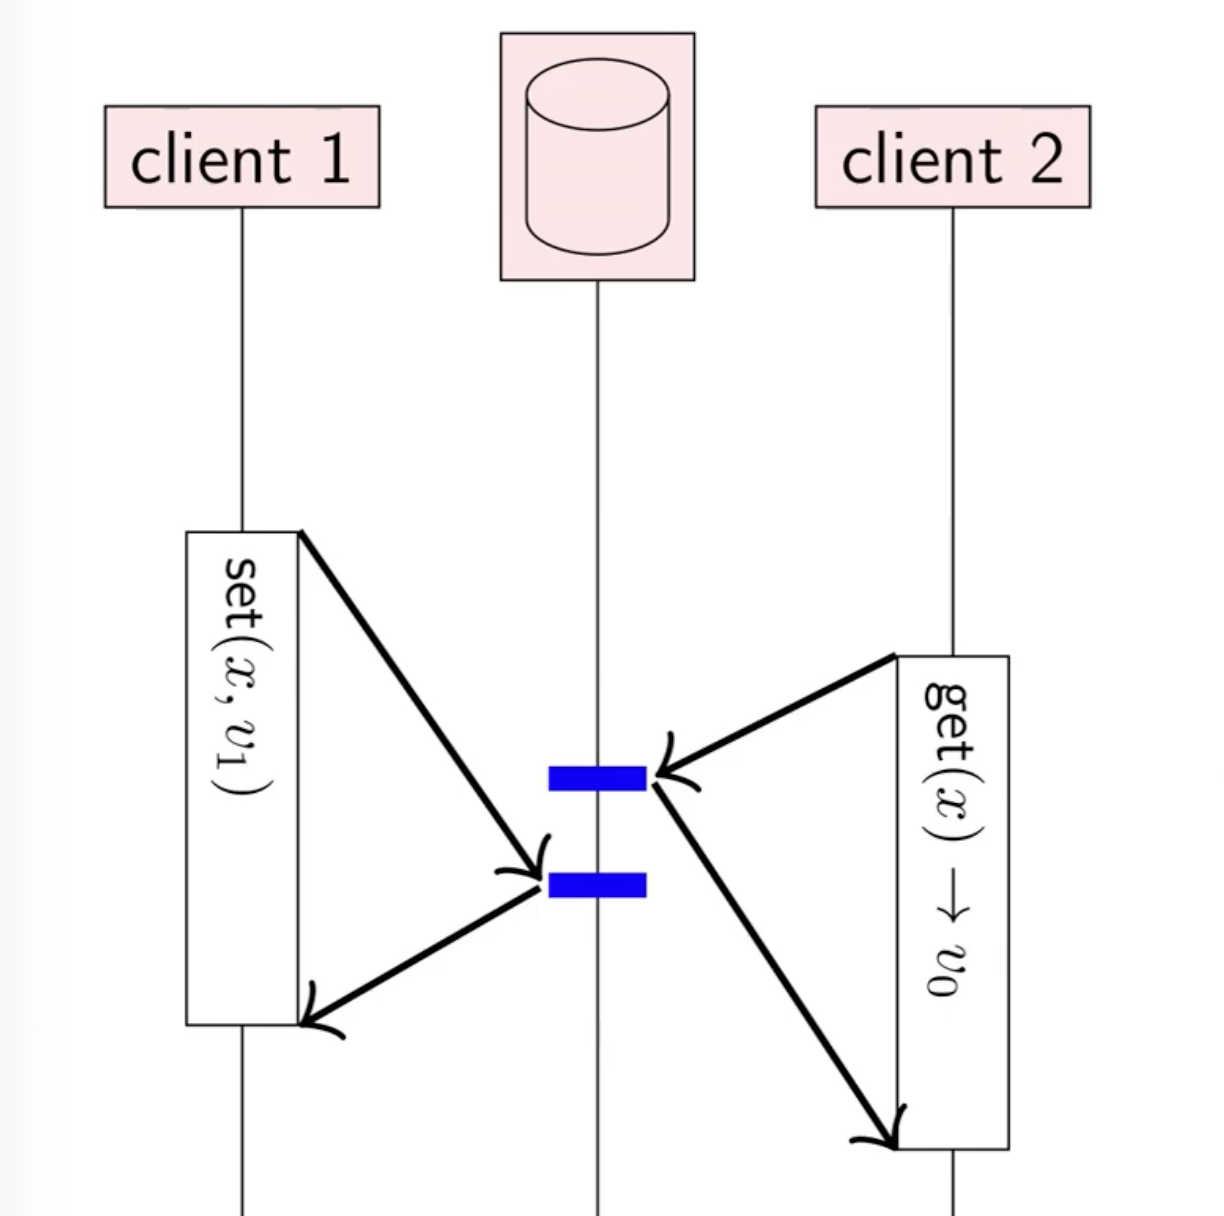
\includegraphics[scale=0.25]{computer-sceince/distributed-media/linearization.png}
        \caption{ If both overlap in time, it is okay that one starts after the other or the other way around
        }
\end{figure}

Some distributed systems do not provide linearization. 
for instance, quorum write, but not quorum read (quorum is performed only by the client).

\begin{figure}[t]
    \centering
    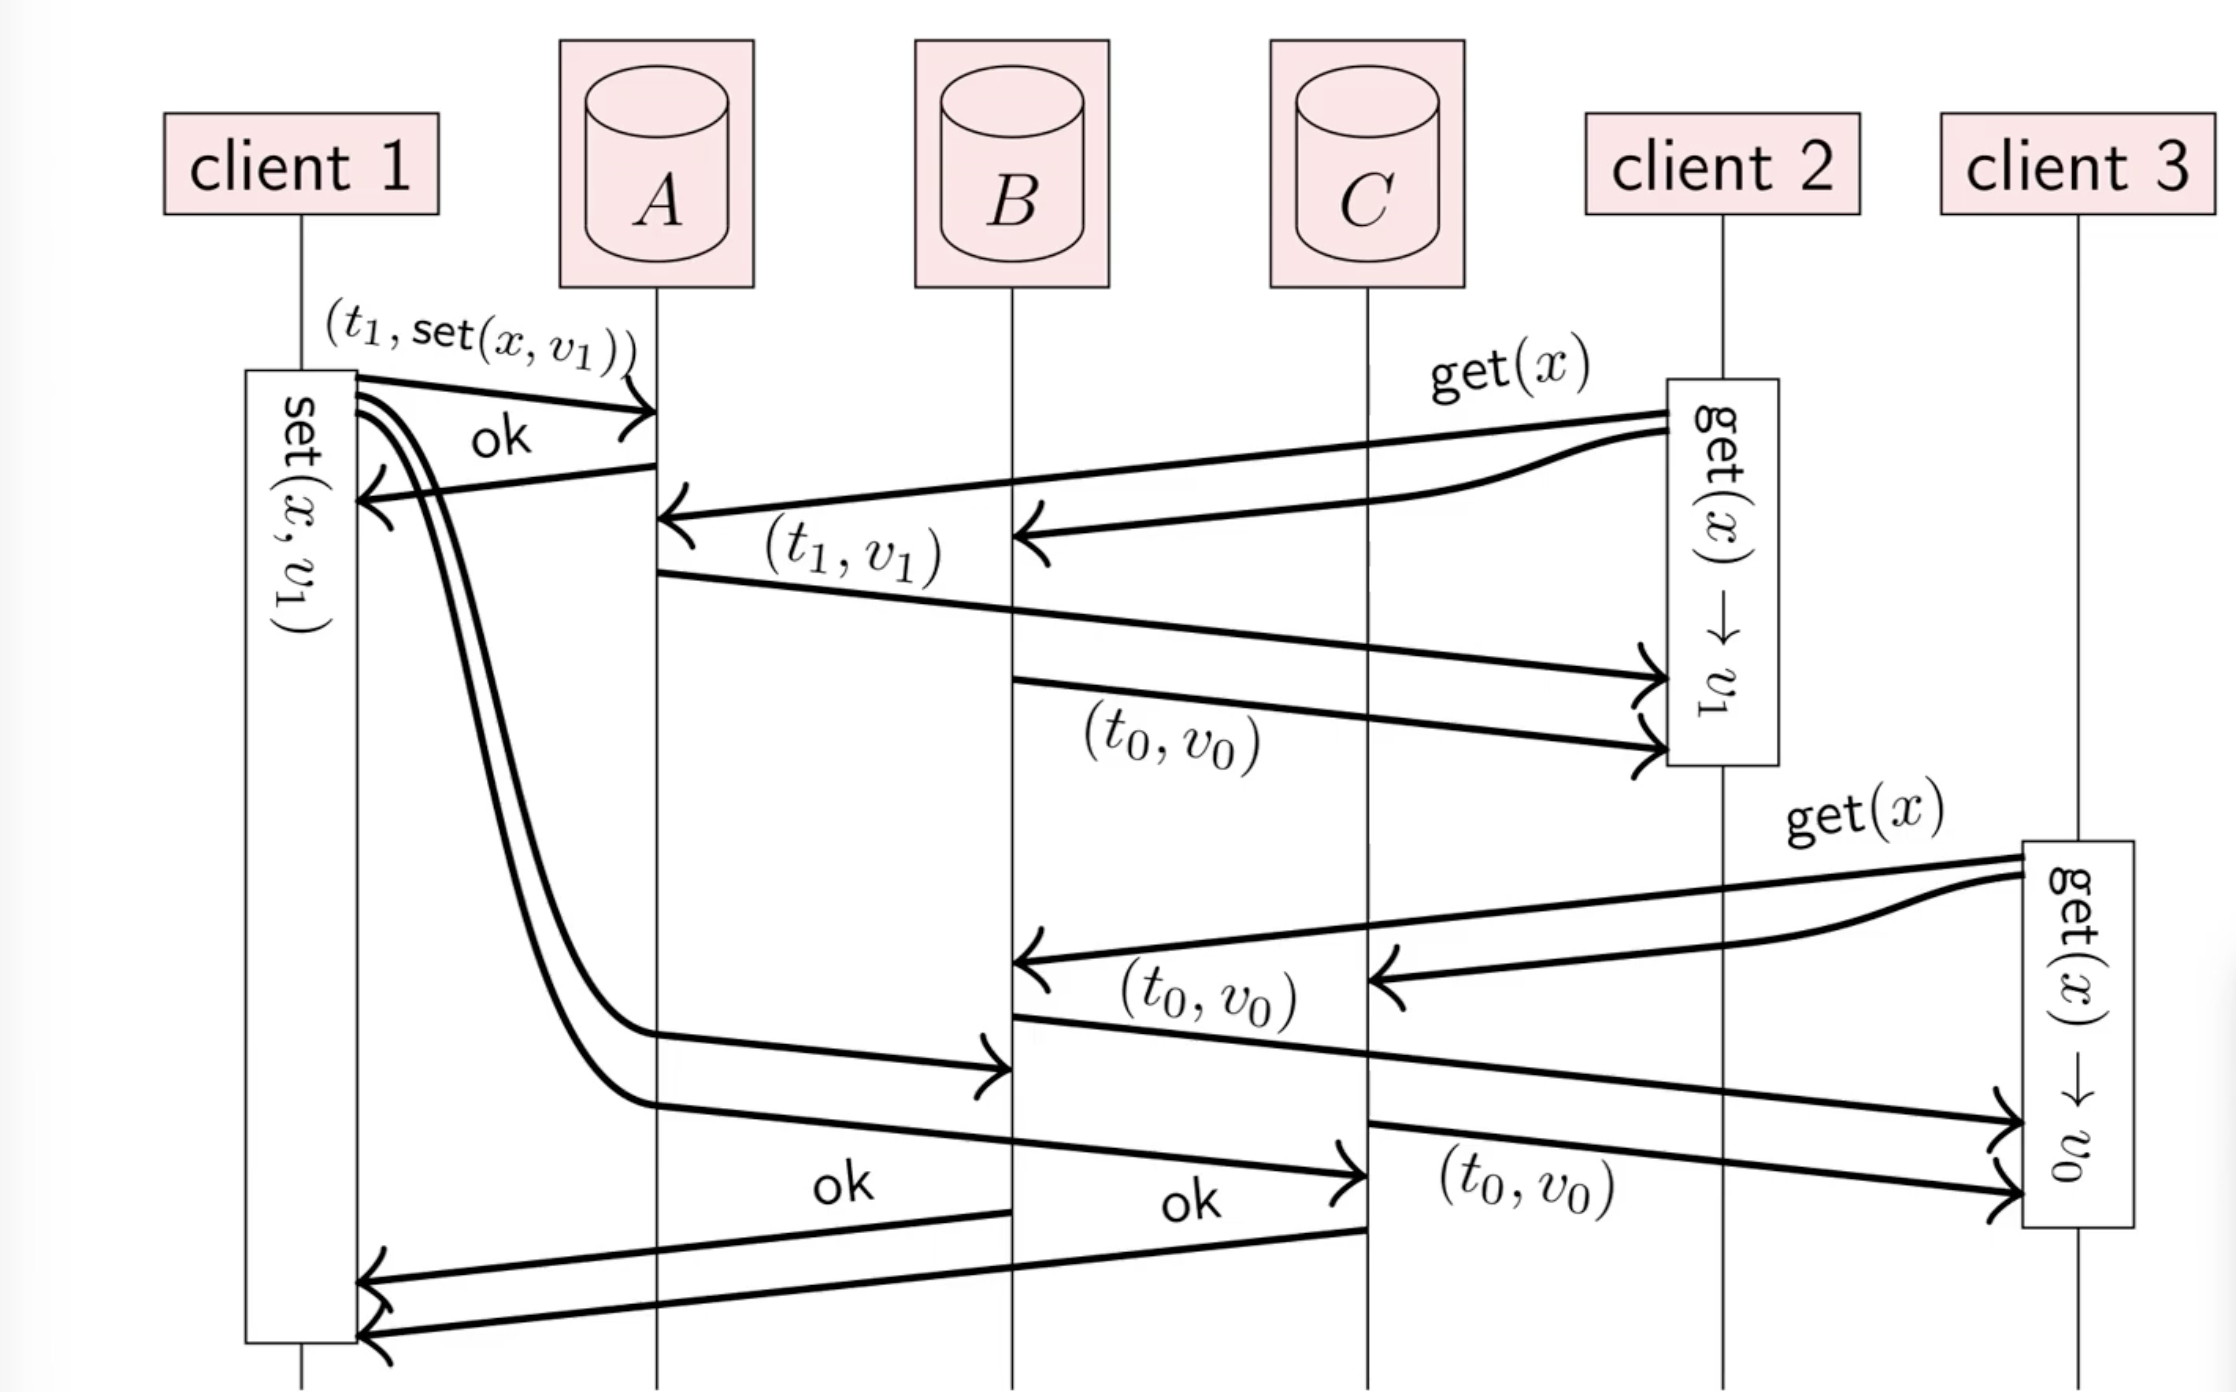
\includegraphics[scale=0.25]{computer-sceince/distributed-media/linearization-failure.png}
    \caption{Notice that $client_3$ started after $client_2$, but got value
    from version $v_0$, while $client_2$ got the value from version $v_1$.
    }
\end{figure}

\todo{could not find formal definition.}



\printbibliography
\end{document}
